% BangorEE - (an unofficial) Electronic Engineering Dissertation LaTeX Class.
% Usage info and bug reports at https://github.com/owenjones/bangoree

\documentclass[msc]{bangoree}

\usepackage{lipsum} % To create some filler content
\usepackage[style=authoryear-ibid]{biblatex}
\usepackage{amsmath}
\usepackage{subcaption}
\usepackage{appendix}

\title{Leksis, an Adaptive Vocabulary Test For Low-Resource Languages}
\author{Alan Kersaudy}
\course{Language Technologies}
\date{September, 2025}
\supervisor{Dr. G. Bovolenta}

\addbibresource{references.bib}


\begin{document}
    \renewcommand{\labelenumii}{\arabic{enumi}.\arabic{enumii}}
    \renewcommand{\labelenumiii}{\arabic{enumi}.\arabic{enumii}.\arabic{enumiii}}
    \renewcommand{\labelenumiv}{\arabic{enumi}.\arabic{enumii}.\arabic{enumiii}.\arabic{enumiv}}
    \maketitle
    \statements
    \abstract{}
    \acknowledgements{
      Any quality that may be found in this dissertation should not be attribued to its autor, who only bears the small responsability of puting together ideas, insights, and reflections from others. Even this small effort was itself directly or indirectly supported by people and institutions who made my stay in Bangor as pleasant, beneficial and productive as it could possibly have been. Especially, I owe a direct debt to Giulia Bovolenta, who first oriented me towards vocabulary testing, and whose many insights guided each steps through this work. Maria Kolesnichenko is the lighthouse of kind common sense that kept me from drowning in a sea of bad ideas during the whole year. Melanie Jouitteau, who first seeded in my mind the idea of doing this Master degree in Bangor. The teaching of Philip Davies in the TSI course who helped me improve my Welsh skills, along with fellow Welsh speaking students that I can only be gratefull to call friends, Leena Farhat, Tom Williams, Stephen Russel and Owen Williams. Preben Vanberg among many things is the person responsible for the idea of placing the items difficulty on the same logistic scale as the test takers. The whole team of the Canolfan Bedwyr, among which Tegau, Cat, Alun, Steffano and many others. But especially its Technology Unit's director Gruffydd Prys and his family, whose effort in welcoming me and supporting my stay in Bangor cannot be given justice with words. Two other teachers, Dewi Bryn Jones and Bill Teahan, who, in a very different but complementary way, helped me to master many of the skills that made this work possible. Finally, the financial support I was given from Cymen is an opportunity that motivated me to produce the best tool I could materially produce for the Welsh language. I ultimately dedicate this test and the tutoring agent associated with it to Cymen and its directors Manon Cadwaladr and Aled Jones as well as Myfyr Prys, for their role in enabling the Cymen scholarship. Let it be small gesture of gratitude for the trust and freedom they've given me. I am blessed and grateful to have crossed the road of so many smart and good peoples and this work is mostly the fruit of their collective kindness.
    }
    \tables

    \content
    \chapter{Introduction}    
    \abbrv{LRL}{Low-resource Language}
This chapter presents the stakes, scope and purpose of the present dissertation. Particularly, the third section brings to light the role that educational technologies have to play in either supporting or further endangering low resource languages (LRLs), depending on whether the technology is meant to teach languages already endangering other languages. This section can be read as a general introduction to the field of educational technologies for those concerned with the fate of LRLs or as an introduction to the concerns of LRLs for those involved in the field of educational technologies.

\section{Structure of the Dissertation}
This dissertation introduces Leksis, a new recognition vocabulary designed test tailored for LRLs. This first chapter explains the rational behind such a test. The second chapter brings together parts of the available literature from different fields ranging from applied linguistics to information theory in order to set the ground for scalable vocabulary tests adapted to the limitations and context of LRLs. The third chapter present an initial test design for the Breton language. The fourth chapter analyses the results from the test to assess the relevance of the design choices. Finally, the fifth chapters assesses the value and limitations of the test, as well as presenting an informed opinion on the needs specific to LRLs in regards to both educational and language technologies.

\section{Aim, Objectives and Research Question}
LRLs face peculiar challenges in a world where data science made quantity the mother of all qualities. The ultimate aim motivating the present work is low resource languages teaching optimisation. The essential problem of any optimisation being the metric one aims to optimize, this lead to the development of rapid, minimalist language tests that will be introduced here. Especially, the objective is to find ways to make up for the resource scarcity problem by developing methods and techniques designed to work in this scarcity context first, rather than porting to LRLs methods and techniques that too resource intensive.\\
For these reason, we propose the following research question.

\textit{Can a quick, adaptive vocabulary test be created for low-resource languages?}

Adaptivity encapsulates both reliability and precision, two key aspects of psychometric validity. So validating adaptivity can be used as a proxy to validate the potential for test to track progress through time, without a large-scale study. Studies that would require following entire groups of learners over several months to gather the necessary results. By studying thoroughly the available literature and assessing the adaptivity of an actual test from its early results, the intention is to support a solid argument in favour or against this idea by the end of this work. 

\section{Background and Motivation}
    \subsection{Terminology: AIED and EdTech}
        \abbrv{EdTech}{Education Technologies}
        \abbrv{AIED}{AI in Education}
Modern academic research on educational technologies primarily falls under the ``AI in Education'' (AIED or AIEd) umbrella. This terminology dominates the field because of the ``International AIED Society'', founded in 1993, and the structuring impact of its journal issues and conferences. However, AIED may at time be used somewhat interchangeably with EdTech, for ``Educational Technologies'', which is a more product and market oriented terminology, a term that relates more to other neologisms like ``FinTech'', ``BioTech'' etc\ldots Educational companies such as Duolingo or Rocket Language may be considered as EdTech companies for the industry, but belonging to the field of AIED for researchers. In yet another formulation, EdTech is AIED with a business model.

    \subsection{Lower Resource Language in Educational Technologies}
        \abbrv{NLP}{Natural Language Processing}
        \abbrv{WEIRD}{Western, Educated, Industrialized, Rich and Democratic}
The question of LRLs in AIED is tightly correlated with their general situation in the field of natural language processing (NLP). The situation is best described in \textcite{magueresse_low-resource_2020}, as statistical, connectionist, methods became dominant in NLP, the question of data scarcity becomes the main limiting factor in the application of modern NLP solutions for LRLs. This problem is also compounded with a general WEIRD bias in cognitive science \parencite{henrich_most_2010}, where languages from cultures that are wealthy, educated, industrialised, rich and democratic tend to be privileged in all fields of cognitive sciences. However, if the adoption of these technologies is the most limited for LRLs, it is ironically these languages that stands the most to lose from not adopting them. Not adopting these technologies can cause a loss of visibility, prestige and desirability, which in turn leads to a lesser adoption and usage, leading to a vicious circle where less training resources are available to adapt these technologies to LRLs. This phenomenon as been described as the digital stagnation, or death, of a language, which is the online signature of socially extinct languages \parencite{kornai_digital_2013}.\\
The role educational technologies could play in breaking this vicious circle, at least for some of the languages concerned, cannot be understated. On the one hand, helping to adapt existing educational technologies to LRLs languages can help to maintain their relevance as a teaching medium for parents who wish the best educational standards for their children and offer people seeking intellectual fulfilment an alternative to simply abandoning their mother tongue to keep learning new things. It is understood that NLP technologies such as automated translation can help to port established educational technologies to a large number of linguistic communities which do not possess the resources to otherwise develop their own educational tools \parencite{haddow_survey_2022}. A study by \textcite{horbach_crosslingual_2024} supports the idea that educational equality can be achieved through cross-lingual scoring systems, in the context where open questions are used to assess skills, and where different linguistic backgrounds may impact the fluency of the students answers regardless of their understanding of the concept assessed. On the other hand, when it comes to language oriented educational technologies, the field is almost entirely dominated by research to teach English, and even coming in concurrence to already endangered languages. A paper by \textcite{henkel_supporting_2025} is symptomatic of those risks.
In this study, English speech recognition technologies are used in an AIED system to improve literacy in Ghanaian schools, a country home to more than 70 indigenous languages \parencite{noauthor_ghana_nodate}.
To the best of our knowledge, it seems that little effort have been engaged in the academic literature to support the development of educational technologies specifically tailored for the needs of LRLs and their speaking communities, despite all the progress made in recent years to develop these languages in NLP\@. This lack of evidence may be caused by a language barrier, but this only reinforce the idea that more should, if must not, be done to support LRLs in AIED\@.

    \subsection{Artificial Intelligence and Education}
    \abbrv{DL}{Deep Learning}
    \abbrv{AI}{Artificial Intelligence}
As exposed by \textcite{doroudi_intertwined_2023}, artificial intelligence (AI) and research in education entertained a 70 years long dialectic that benefited the two fields of cognitive sciences. If early works on AI initially drew from developmental psychology and even developed educational tools as part of their endeavour to emulate human intelligence with machines, it is now the field of education that benefits from the possibilities unlocked by AI technologies.

Early research in artificial intelligence explored two different approaches to try to emulate cognitive processes. The first is commonly known as Good Old-Fashioned AI (GOFAI\abbrv{GOFAI}{Good Old Fashioned AI}), it was centred around a symbolic approach that stemmed from Allen Newell, Herbert A. Simon and Cliff Shaw's seminary work on the Logic Theorist \parencite{newell_logic_1956}. This approach sought to understand how experts solve problems using rules-based systems and symbolic abstractions. The second, connectionist, approach was centred around neural networks and focused on the acquisition of cognitive skills over performance proper. It was developed by people like Marvin Minsky, Seymour Papert and many others \parencite{doroudi_intertwined_2023}. Papert notably, came to the AI world after having studied children cognitive development in Jean Piaget's laboratory in Geneva. He brought to the connectionist paradigm in AI a consequent influence from Piaget's constructionism, which is a theory that posits that learners build their skills and understanding on the knowledge and skills already acquired.

Both approaches led to attempts to create interactive educational systems early on. Examples of early educational software programs based on GOFAI comprise the GUIDON system, which relied on the Mycin engine, an infection diagnosis system, to teach students diagnosing pathologies \parencite{william_j_guidon_1983}. The connectionist branch privileged the development of educative "micro-worlds", such as educative programming languages, in which children could learn unspecified problem-solving skills. Instances of such approach comprise the Logo programming language, designed to learn about relative positioning and geometry by designing programs to guide (drawing) robot turtles. Many systems followed Logo, like the Scratch programming language and the Lego Mindstorms kits. But the necessary specialization in AI led later research to strictly focus on computer systems performance, especially as the advent of back-propagation gave rise to deep learning (DL), achieving to establish the supremacy of the connectionist paradigm in AI.

At this point, the focus definitely shifted from using developmental psychology to support AI, to integrate AI technical solutions in educational tools. A meta-analysis by \textcite{schmid_meta-analysis_2023} now supports the benefits of constructivist educational approaches like Blended Learning (BL) \abbrv{BL}{Blended Learning} and the Flipped Classroom (FC) \abbrv{FC}{Flipped Classroom}, which give more of a coaching role to teachers, with the charge of the instruction being deported to online interactive systems, most often used outside the classroom.

In this section, we saw how Piaget's constructivist ideas in education first infused in the connectionist approach to AI through Seymour Papert's works. Then, when this connectionist approach took the world by storm with the advent of DL, AI came back to education in the form of adaptive learning platforms to support constructionist practices development in schools. Learning about this combined history goes beyond a mere inquiry for historical anecdotes, it gives us the scope and epistemological framework to fix the goals and methods of educational technologies, which is a necessary step to ensure that such tools could one day achieve real-world success. This is, not as an isolated system evolving in the vacuum, but tools in the service of a holistic learning environment.
    
    \subsection{Adaptivity and Knowledge Models}
        \subsubsection{The Promise of Adaptivity}
The key difference between classic textbooks or lecture-based education and most of the recent learning technologies is the promise of adaptivity. This means that the system adapts its behaviour based on the learners' performance, ideally with the goal to maximize their learning intake. In most modern systems, but not all, this maximization is done by a recommender system, the most sophisticated forms of which resolve an instance of the multi-armed bandit problem. Problem which may be solved by one of several different algorithms \parencite{chen_recommendation_2017}. The multi-armed bandit problem is the mathematical formulation of a situation where different actions are proposed, in our case, recommending different learning materials with uncertain pedagogical values, and an agent must decide which actions will maximize a specified reward, here, the students' growth in knowledge. Those systems must make an arbitration between exploiting actions with known, but limited rewards and exploring actions with unknown rewards.

This paradigm allows systems designers to free themselves from the headache caused by having to arbitrate the question relating to the selection of learning material, like their relative difficulty; one exactly on par with the level of the student, or one leveraging other teaching paradigms such as desirable difficulty, or a combination of the two. Depending on the algorithm selected, the promise of adaptive learning is to enable the construction of an individualized profile of the learners' skills, possibly also including a description of theirs learning capacity or rhythm, and to have the system build an optimized curriculum to reach the specified pedagogical goal.

It must  be pointed out that more rule-based systems still exist, and are widely implemented, where the curriculum is designed in advance based on a pedagogical model, playing the role of the recommender systems presented above. Those systems may be relevant when the goal is to teach a specific, well-defined, sets of skills, like primary and secondary schools programs. \textcite{pelanek_adaptive_2025} mentions the Umíme platform in the Czech Republic, that seems to be largely adopted by schools and relies on such architecture. Others systems may not even have adaptivity systems, but simply interactive properties, like the educational programming languages mentioned above, but those are not the focus of the present work.

        \subsubsection{Knowledge Model and Instrumental Goal}
Where recommender systems can make the promise to optimize any given metric, from a YouTube video watch-time to paperclip manufacturing \parencite{bostrom_ethical_2003}, AI systems do not bear the responsibility to define these intermediary instructions, what we call the instrumental goal. This question is at the core of all alignment considerations, and educational systems are no stranger to this probematic. In educational systems, this proxy is based on a knowledge model, also called student model, which are psychometric data from which can be derived a learning model (the evolution of that knowledge through time) which may in turn be used to define the pedagogical value of a teaching material, this metrics being the reward that a multi-armed bandit algorithm would be charged to optimize. The definition of this knowledge model and the nature of the psychometric construct it collects is quintessential to the success of an adaptive learning system, and this definition is the responsibility of the field that the system is intended to teach and psychological models, not AI directly.

    \subsection{Conclusion}
In this section, we analysed the history of educational technologies since the cognitive revolution in the 1950s. We saw the invaluable potential of the still emerging field of AIED, and its promise of adaptivity, together with the risks and opportunities it brings to LRLs. We identified a gap in the literature on LRLs teaching in AIED. If the translation of AIED systems in LRLs may work as long as the topic it is intended to teach is not a language itself, when it comes to teaching languages, the innovations in the field of language educational technologies seems dominated by English, which is an outlier in terms of resources' availability when compared with the majority of the 7000 other languages spoken around the globe. In this context, it seems necessary to rethink how adaptivity can be achieved when most languages around the world don't even possess a scientific descriptive grammar, let alone the dozens of hours of annotated recordings necessary to train speech recognition systems.


    \chapter{Literature Review}

This literature review is divided in two main sections. The first section is dedicated to the analysis of the constructs that have been investigated in assessing language proficiency, and among those, which ones could serve in an adaptive learning system, while the second one dwell on the statistical ways to score and analyse a given construct. The guiding criterion throughout this chapter will be the simplicity of the solutions proposed, because, in any case, it is always easier to fix a simple system's shortcomings than those of a complex system.

\section{The Proficiency Constructs and Where to Find Them}
    \abbrv{LS}{Learning Science}
    \abbrv{SLA}{Second Language Acquisition}
The introduction exposed how the definition of the instrumental goals that a recommender system has to optimize belongs in the domain of expertise relating to the final goal of the system, rather than in the technology itself. Language testing has traditionally been the matter of Second Language Acquisition (SLA) research, which can be seen as a subdomain of learning science (LS), but this field takes inputs from – and is closely related to – psycholinguistics, applied linguistics, and as we shall see, neuroscience, on which it depends for a general understanding of the processes involved in language use and acquisition. Without pretend to an exhaustive review, this section will attempt to provide a unified overview of language proficiency and the ways to measure it.

This question has been widely studied within various theoretical frameworks and for several practical purposes. Most noticeably, on the mastery of a language can depend the access to citizenship, educational institutions or work positions, which are live-making opportunities that have made its validation a social mobility issue. In this section, we start with the most widely accepted and used way to assess language skills, before moving towards alternative solutions that would fit the needs of a scalable adaptive learning system. Finally, we critically assess these alternatives. The second section is dedicated to finding ways to address the shortcomings of these alternatives.

    \subsection{The Holistic Approach to Testing (CEFR)}
        \abbrv{CEFR}{Common European Framework of Reference for languages}
The complex latent traits like language proficiency can be assessed by two testing paradigms, the first being described as maximalist, comprehensive or holistic, and the second minimalist, proxy-based or reductionist. Commercial and institutional language tests such as the IELTS and the Cambridge English Qualifications for English or the DELF and DALF for French, to only cite these, follow a maximalist approach defined by the Common European Framework of Reference for languages (CEFR) \parencite{europe_common_2020}. This framework not only define the now famous six alphanumeric degrees of language mastery, but also the four usage contexts in which it ought to be measured, two modes of usage, oral and written, for two types of activities, reception and production. It measures the linguistic knowledge (vocabulary, grammar and their constituents) together with the four common language skills that language users engage with: listening, speaking, reading and writing. This framework is considered standard beyond the borders of Europe, but in spite of its strengths, it may not suit all contexts in which languages need to be tested.

The main critique that could be levelled at this testing paradigm is the fact that only ten European languages can brag about having CEFR-compliant tests spanning the six proficiency levels it defines \parencite{noauthor_common_2025, noauthor_cadre_2025}. After twenty-five years of existence, even national languages of leading economies of the EU like Dutch or Czech, do not belong in this list. This is a fundamental flaw for a paradigm that was explicitly designed not to favour the main languages of the Union. The reasons for this are obvious, only the most ``marketable'' languages can develop an educational ecosystem strong enough to make these tests economically viable. Sometime, political will can breach the gap like for Spain's regional languages (Galician and Catalan are in the ten languages mentioned above, when Basque only lacks a test for the A1–2 levels), but this will is built on strong institutions and expertise that only a handful of languages have at their disposal in Europe, let alone in the rest of the world. Despite its theoretical grounding, the scarcity of resources (time, money, expertise and interest) make a comprehensive language testing paradigm impractical for most languages, which are once again left behind. Once again, it is the languages that have the most to benefit from these tools, and the most to lose by not using them, that are facing the greatest difficulties to access them. Furthermore, in the case of an adaptive learning system, which is the main motivation for this dissertation, a comprehensive test would be both redundant and unpractical, as the testing would take too much time from the learning experience, unless the testing were to be part of the pedagogy.

We must thus look at more efficient ways to measure proficiency, but before this, we need to develop a deeper understanding of what language acquisition means, how the abstract theoretical knowledge present in the unread dictionaries and grammars articulates with the two or four practical skills that characterize daily language use of all known human cultures around the globe. What is competence and performance in regards to language proficiency?

    \subsection{The Intertwined Nature of the Proficiency Constructs}
Most theories in linguistics, especially de Sausure's structuralism and Chomsky's generativism, are based on an analytic approach, first taking language in isolation from other mental processes, then separating its conceptual constituents, lexis from grammar, competence from performance \parencite{chomsky_aspects_1965} and repeating process with their constituents and subconstituents, to then study the ways to combine them together. In a way, the CEFR paradigm follows the same epidemiologic trend, by dividing production and perception skills, oral and written usages. The main benefit of these analytical methods is obvious, by separating aspects and categories, one can cover an exhaustive understanding of the constituents and rules of a complex systems such as languages. But despite its strength, this analytical approach brings a biased view as to what a language is, as it brings a static and isolated representation to the systems it studies. However, languages, or for this matter language knowledge, never are a fully static structure nor a succession of synchronic states, because languages live the human flesh, they have to be acquired and forgotten by every passing generation and are never stagnant, nor limited to their internal structure. This is where modern approaches, like functionalism or cognitive linguistics \textcite{evans_cognitive_2009} come into play, along by developmental psycholinguistics, by bringing the focus to the acquisition and use of the language and it's relation to the body, rather than its structure.\ \textcite{bybee_usage-based_1999} argues that usage-based linguistics can produce formal models, but with a twist. By stating that the competence comes as the formalisation of usage, almost as an emerging property, and this usage of the language being primarily a social, physical, embodied and cognitive activity, this new paradigm brings new considerations into light. Where generativism view performance as the materialisation of innate structures of the brain giving the structure precedence over anything linguistic, usage-based approaches consider structures as generalisation made by the language learning brain. This view goes beyond the simple inversion of precedence in what is an obvious chicken-egg situation. By insisting that cognitive processes always have some degree of dependence on embodied, sensorimotor processes, this view also breaks the Cartesian mind-body duality \parencite{varela_embodied_1991} as well as Chomsky's competence-performance duality. In simple words, everything in the brain is (or eventually becomes) connected based on usage, and structures always come a posteriori.

These developments in linguistics proper are also supported by recent advance in neurology. Since their discovery by Vermon Mountcastle in the 1950's, it has been debated whether the cortical columns inuformally structuring the the grey matter in the neocortex play a role as a modular unit of computation \parencite{horton_cortical_2005}. The thousand brains hypothesis \parencite{hawkins_theory_2017, hawkins_thousand_2021} is the latest iteration of this idea and proposes a model on how this unique architecture can, through a voting mechanisms, progressively map sensorimotor inputs towards and from different degrees of abstractions and to refine a unified representation of the world, and thus better engage with it in a continuous feedback loop. This produces a compelling argument on how abstract thinking and language can progressively emerge from sensorimotor interactions \parencite{constantinescu_organizing_2016}, when Chomsky's genes of a Universal Grammar are still waiting to be found anywhere.

        \subsubsection{Implications for Language Testing}
        \abbrv{L1}{First Language or Mother Tongue}
        \abbrv{L2}{Second Language}
At this point, the parallel between the CEFR testing paradigm and formal linguistics has to be clarified, because in the CEFR paradigm, in a way, we measure performance to deduce competence, so the link between those is never denied. But the epistemological critique of the quest exhaustiveness as undermining the understanding of the dynamics of the acquisition process still stands. If we are interested in the acquisition process and its dynamics, a complete, static representation of the skills is counter-productive. Furthermore, if the competence does not exist independently from the performance, could the skills be deduced from knowledge itself? This is what functionalist linguistics seems to argue for.

If everything is connected, if all is one (though one is not all), that is, if more practice leads to better practical skills, or performance, which leads to better theoretical knowledge, or competence, then, performance could in theory be measured through any construct describing competence, such as vocabulary knowledge. Vocabulary is especially interesting as its acquisition is a discrete, yet, never-ending process during a language learning journey.\ \textcite{eun_hee_jeon_understanding_2022} published a series of meta-analyses on the correlates of the different practical skills defined by the CEFR, all pointing towards this direction, with vocabulary knowledge being cited as a strong correlate for proficiency in listening \parencite{innami_meta-analysis_2022}, speaking \parencite{jeon_meta-analysis_2022}, reading \parencite{jeon_updated_2022} and writing \parencite{kojima_meta-analysis_2022}. Note however that this does not mean that vocabulary knowledge causes fluency, although it contributes to it to the extent that fluency does not come without an advanced level vocabulary knowledge. This basic premise opens the door for low stake, low-cost, LRLs-friendly quick testing which may be more scalable and applicable in many areas, from self-assessment, to the development of automated language learning tracing systems mentioned in the introduction. Notably, in the context of LRLs, that some may call ``oral languages'', the idea that higher vocabulary level is linked to practical skill becomes even more likely, because the dominant way to access knowledge is a ``more integrated usage'' (one doesn't learn Rapa Nui in the books). This way, one may even posit that vocabulary testing becomes increasingly relevant as less written and digital resources are available to a given language. 

The last implication of this first-principle and connectionist view of language acquisition is the absence of practical difference between the way competence in the first language (L1) and a second language (L2) are acquired, that is, through usage. Once the circuitry responsible for verbal communication is unlocked between age 1 and 6, either through monolingual (including a sign language) or multilingual education, the way new words are acquired is consistent across the languages spoken by a multilingual. If a word or a feature is discovered through integrated usage and the piece of knowledge in the brain stems from a sensorial experience present during the acquisition of the term, and if a word in L2 is learned as the translation of a word in L1, its representation in the brain will stem from the L1 word as its synonym within another ``register'' which is the network of the L2. The two scenari implying a formation of knowledge from the usage context but with no difference in status between the L1 and L2 networks. A word can be learned in L2 as the product of an integrated experience, and its L1 equivalent can be learned at a later stage as a ``synonym in another space''. As someone who learned about back-propagation in English first, my third language, I can assure the reader that I still need to think about the English word before finding its translations during a conversation in French or Breton. Once again, this equivalence between L1 and L2s is convenient in the context of LRLs, because these languages are often the low variety in diglossic regions, where the notion of native speaker and the line between L1 and L2 are often blurred.

    \subsection{A topography of Vocabulary Tests}
It has often been shown that well-chosen proxies can give a reliable understanding of complex processes that one tries to measure. Economists have for example shown how nightlight measurement from space can serve as a reliable growth indicator in countries where official statistics may be lacking in quality or honesty \parencite{henderson_measuring_2009}, even without providing a causal mechanism for why this may work. Linguists imagined many ways to define and measure vocabulary knowledge, as they understood and demonstrated the strong correlation it had with other constituents of language proficiency. This last part of this first section of the literature review will give an overview of the different ways linguists attempted to measure vocabulary so far.

        \subsubsection{Productive Vocabulary Tests}
The most integrated ways to test vocabulary consist of asking the test takers to give a synonym of a word, thus assessing the productive vocabulary skills, the words that the testees can, not only recognize and understand, but also retrieve from its meaning only. It is one of the strategies used to measure the vocabulary index, which is combined with three other indices to calculate the so-called IQ of the test taker in the Wechsler adult and children intelligence scales \parencite{wechsler_wechsler_nodate}.

        \subsubsection{Receptive Vocabulary Tests}
        \abbrv{VLT}{Vocabulary Levels Test}
In the middle are found a series of tests that aim to measure receptive vocabulary skills, the words that can be associated with their meaning by the test takers. The most widely used of those is the Vocabulary Levels Test (VLT), developed in the 1980s by \textcite{nation_teaching_1990} (see~\cite{kremmel_vocabulary_2017} for more details on its implementation, evolution and application). This test was designed for widespread use in schools as a placement tests for students. VLT is somewhat adaptive too, as it is testing the skills to associated terms related in meaning from different frequency ranges. An interesting receptive vocabulary test design is the Peabody Picture Vocabulary Test \parencite{dunn_ppvt-4_nodate}. As it is based on pictures instead of written words, it allows testing children who could not otherwise read the words assessed. This picture-based approach could seem to make this testing design an ideal candidate for translation, and thus a candidate for a universal standard that could be applied even in environments where literacy is not widespread. However, this idea may be good only on appearance, as the calibration for the pictures-words mapping took place in an English-speaking country, and the words that may be used to describe similar situations may vary greatly between different linguistic spaces. This is what \textcite{kartushina_use_2022} learned the hard way as they tried to translate the test in Russian for preschoolers, somewhat accidentally demonstrating that the Peabody test may be one of the hardest vocabulary tests to port to other languages, even ones spoken in a somewhat WEIRD society like Russia.

        \subsubsection{Recognition Vocabulary Tests}
        \abbrv{LDT}{Lexical Decision Task}
        \abbrv{SDT}{Signal Detection Theory}
Finally, the simplest family of vocabulary tests are recognition vocabulary tests, sometime simply called simple vocabulary tests, they measure the aptitude to merely recognize the presence of a word, without requiring the justification of a further understanding of the meaning of the word. For an overview and assessment of different designs, see~\cite{meara_complexities_1994}. The most successful design of this vocabulary testing family are the lexical decision task (LDT) vocabulary test, they were given many other names such as ``Yes/No'' or ``binary'' vocabulary tests, but all follow the same principle; a sequence of testing items, either real words of a pseudo-words \parencite{meara_imaginary_2012} are presented to the test takers, who is systematically asked whether they think the item belongs to the lexis of language concerned. The results come in a combination of the four output defined by a confusion matrix, hits, misses, false alarm and correct rejection and different methodologies have been proposed to treat the results, from subtracting the percentage of the wrong answers from the percentage of correct answers, up to applying more complicated systems from Signal Detection Theory (SDT) \parencite{huibregtse_scores_2002}.

Many such tests have been built so far include at least one online version, and, encouraging fact, available in several languages English, Dutch and German \parencite{lemhofer_introducing_2012}. This paper showed encouraging results, with strong correlation of the vocabulary result with other traditional tests, thus supporting the idea that proficiency can be effectively measure through vocabulary testing. Another test has apparently been made for Croatian \parencite{srce_how_2025}, although more information is not yet available. And this is in parallel with the numerous systems developed by Meara over the years\cite{meara_complexities_1994}. The main limitation of these systems is the fact that their items are limited and static, so they are never designed for a repeated usage, which would help measure the dynamics of vocabulary acquisition. This is a problem to be fixed, because the main interest of a minimalist test is to allow recurrent testing.

    \subsection{Relevance and Limitations of Vocabulary Tests}
All the vocabulary tests presented above had their load of commercial or academic success due to their reliability in capturing different aspects of vocabulary acquisition. This shared reliability even works against the idea of seeing any of those becoming a standard, because they would all play an equally relevant part in this matter. We already explained the reasons why this should be so in section 2.1.2. If one admits that any sub-construct of proficiency is linked in the brain in a way defined by usage, that ``all is one'', then the same logic applies to vocabulary. Recognition comes as the first stage of vocabulary acquisition, without which any further development towards a more integrated usage is impossible. All these testing families measure different stage of the same integrated process of vocabulary acquisition. Nightlight measurement does not only measure the ``nighttime electric consumption dedicated to street lightning of a territory'' construct, but, as the statistics showed, it can be used as a GDP indicator, which is itself an indicator of economic health. The same goes for these vocabulary tests, they all are different constructs measuring the same phenomenon of vocabulary acquisition, which is an integral part of language acquisition.

The main differences between these tests are how resource-intensive they are and how integrated the constructs they measure are. Simple indicators like mere vocabulary recognition have weaknesses and can be subject to cheating or manipulation. The Economist's famous Big Mac index for inflation was allegedly the target of manipulation attempts by the Argentinian government in 2011 \parencite{politi_argentinas_2011} for this very reason. Similarly, the simpler to acquire a construct used as an indicator is, the more likely it is to become subject to manipulation attempts. But this does not mean that the construct as no value, indeed, both nightlight levels and Big Mac prices are still used today, but in scopes and at stakes relevant to their complexity. The same goes for psychometrics. In the context of vocabulary tests, the Peabody picture test's resource intensive design requirement make it need commercial use to support its complex development. The other, simpler tests achieve only academic success because they are so simple to put in place that they never need commercialisation, which limits their scaling potential and in turn their development. Nonetheless, they are all equally useful in measuring their respective stages of vocabulary acquisition.

    %\subsection{Considerations on Construct Validity}

    \subsection{Conclusion}
In the context of an automated and adaptive testing with the purpose of tracing the acquisition of language skills, the vocabulary tests advantages outweigh largely other methods, and among them, the simpler vocabulary recognition tests designs truly shine, especially when considering the problem posed by LRLs. LDT vocabulary tests are simpler to administer in a fully automated way, and they are easier to port to LRLs because they can be derived from a simple list of dictionary entries. Yet, significant challenges remain before enabling a widespread implementation of LDT vocabulary test. The main limiting factor being the number of items proposed in tests like LexTALE, both real and pseudo-words had to be selected from a larger set during a preliminary study in \parencite{lemhofer_introducing_2012}. If an LDT vocabulary test is to be used in a recurrent way, to trace vocabulary progress through time, the items available for testing must be plentiful, maybe cover the whole lexis of a language or at least a significant portion of it. But then the question of the items calibration kicks in. There can be no question of thinking of scaling the preliminary study done for selecting the items in LexTALE to get enough items to allow reliable recurrent testing, already for a language with tremendous resources like English, let alone LRLs. Solving this problem of the items calibration would open the door to scaling both vertically (allow recurrent testing for the same language) and horizontally (allow porting the test to many languages). The next section will be dedicated to finding such a solution.

\section{Knowledge Tracing}
    \abbrv{KT}{Knowledge Tracing}
    \abbrv{CAT}{Computerized Adaptive Testing}
To paraphrase \textcite{meara_complexities_1994}, many assessment tasks may be valid ways to assess vocabulary recognition skills, be provided the appropriate method of analysis. This section is dedicated to this problematic. Measuring latent traits from a tests items responses is a complex task known as Knowledge Tracing (KT) \parencite{shen_survey_2024}, which is a fundamental concept in Computerized Adaptive Testing (CAT). Part of this complexity depends on the assumptions one makes on the latent traits, are they a continuous construct or a set of discrete skills, which combine together in a multidimensional knowledge space, and if so, which skill depends on which others? These dimensions and the relationships between them can be defined manually or based on data, using Bayesian techniques or DL\@. Other assumptions may include the influence of the testing process on the learning process, in which case one may factor in the half-life of new memories formed during previous assessment rounds. Fundamentally, this complicated choice of the model is an arbitration between accuracy and interpretability \parencite{pelanek_adaptive_2025}. More qualitative models may be appropriate to inform recommendations of learning material, but presenting a proficiency vector as the result of a stand-alone test may be less interpretable than a classic score.

Since this dissertation primarily focus on testing, a unidimensional, quantitative index seems more appropriate.  Furthermore, the calibration of a qualitative paradigm would require large amount of data or resources like time and expertise, which are unavailable for LRLs. The end of this chapter will lay down the theoretical basis a this quantitative interpretation of the results of a LDT vocabulary test.

    \subsection{Theoretical Capacity of a Noiseless Unidimensional Test}
The goal of the knowledge tracing model in a CAT is to make predictions on the outcome future test items in order to select the items whose answer are the most uncertain based on previous results. In the information theory jargon, this is called maximizing the entropy, which maximizes the gain of information by the model by minimizing its uncertainty. Drawing from \textcite{shannon_mathematical_1948}, one can define the theoretical absolute capacity of a noiseless binary test, before adapting it to a noisy environment. In a simple, unidimensional scale, finding this spot of highest uncertainty can be achieved with the binary search algorithm. Take a list of items ordered by difficulty, take an item in the middle,  repeat the the process with the second half of the original list if the answer is right, else, with the first half. Repeat the process until the list is one item long. This algorithm has a time complexity of $\theta(\log{n})$, which means that for $n$ number of items, $log_2(n)$ steps are required to reach the last item. This is 10 items need to be tested for a scale containing 1 024 items, 11 for 2 048 items, 12 for 4 096 and so on...

Supposing that all the words in a dictionary of 30 000 words could be ordered by "difficulty", and that half the items of a test have to be pseudo words to deter cheating, a test using this algorithm would find the test taker's current level in only 30 rounds of testing, to compare with the 60 items used by a test like LexTALE \parencite{lemhofer_introducing_2012}. Even if we take into account the need for error corrections, the total number of step required will remain a proportional to this logarithmic progression. This setup has obvious limitations that we will address in the following subsection, but it bring interesting insights concerning the scaling problem of previous tests. Primarily, it is possible to test a really large number of items in a time efficient way, which opens the door to using the whole lexis of a language as testing items, rather than a selected list of words. This possibility in turn opens the door to unique testing experience, where the chances of going twice through the same testing experience are virtually non-existent. This unlocks the vertical scaling problem that was highlighted earlier in this chapter.

    \subsection{The Elo Rating System}
        \subsubsection{Elo rating and Rasch Model}
        \abbrv{IRT}{Item Response Theory}
        \abbrv{HRL}{high-resource language}
The first obvious limitation of the model previously proposed is the calibration of the items. One cannot get the relative difficulty directly from a dictionary, and the order in which words are acquired by learners may vary greatly depending on various factors. Most vocabulary tests go around this problem by grouping the items by frequency ranges \parencite{nation_teaching_1990, meara_complexities_1994, dudley_context-aligned_2024}. However, possessing frequency lists is often a high-resource language's privilege, and most LRLs don't have such resources at their disposal. For this reason, we propose that the difficulty rating of the words items be directly updated based on the results of the test.

In standardised test, this calibration of the items difficulty if achieved by Item Response Theory (IRT), which is a set of models derived from the Rasch model \parencite{rasch_probabilistic_1980}. The maths behind the Rasch model were rediscovered many times, including outside of the psychometric world, like in chess with the Elo rating system \parencite{elo_uscf_1961, elo_rating_1986}. The key equations for these models are presented below.

\begin{figure}[h]
    \centering
    \begin{minipage}{0.45\textwidth}
        \centering
            $$P(X_{AB} = 1)=\frac{1}{1+e^{R_b-R_a}}$$
        \captionof{figure}{Rasch formula}
    \end{minipage}
    \hfill
    \begin{minipage}{0.45\textwidth}
        \centering
            $$P(X_{AB} = 1)=\frac{1}{1+10^{\frac{R_b-R_a}{400}}}$$
        \captionof{figure}{Elo rating system}
        \label{Elo}
    \end{minipage}
\end{figure}

In the Elo rating system, $P(X_{AB} = 1)$ is the probability of player A of rating $R_a$ winning by checkmate against a player B of rating $R_b$. In the Rasch model, $P(X_{AB} = 1)$ is the probability of a test taker of rating $R_a$ to successfully answer at a questionnaire item of difficulty rating $R_b$. Since both follow a logarithmic progression, the rating from a "Rasch rating" to an Elo rating is done by multiplying it by $400/ln(10)$ and inverting the nominator and the denominator to go from Elo to Rasch. The difference in the logarithm base and the addition of a spread factor of 400 in chess was meant to increase readability and interpretability, while matching rating systems previously used in the chess world. A 400 difference in Elo rating means a 1:11 vs 10:11 chance of victory, which is more interpretable than a 1 point difference meaning a 1:2.718 versus 1.718:2.718 odds distribution.

In practice, the main difference between the two systems lies more in the update mechanisms. Since IRT was developed for static tests (without real time adaptive features), it relies on more computationally intensive techniques, which are not well suited for the purpose of a CAT. Its simple updating system is why the Elo rating system has been gaining more attention in the AIED community over the years, \cite{pelanek_applications_2016} mentions several successful integrations of this model in adaptive educative setups, although never for stand-alone tests. The same article also present various update mechanisms that take into account different assumptions, such as correction for cheating strategies or short and middle term memory half-life. The update of an Elo rating is given by the following formula.
\begin{equation}
    R_{A}^{\prime}= R_A+K \times{(S-P)}
    \label{Update Elo}
\end{equation}
The actual score (1 or 0) $S$ is subtracted by the prediction $P$ of the outcome based on the score difference given in \ref{Elo} (value between 0 and 1). If an outcome is certain (more than 800 rating difference) and the result follows the prediction, this value will be close to zero and the change in rating will be close to 0. If the opposite happens, the score increases by a value close to $K$, names the K-factor a value akin to the learning rate in the DL world. This value that may vary depending on the implementations of the rating system, but is often around 20 in the chess world. Sometime, an uncertainty function is used to progressively change the rate of update based on the number of updates (cf. equation \ref{uncertainty-function}).

        \subsubsection{Error Correction and Degeneracy}
MCQ use three category of component, queries (the questions), keys (the right answers) and distractors (the wrong answers). Fundamentally, recognition vocabulary tests are a subset of MCQs, with a unique query for the whole test, and the real words as keys and the pseudo words as distractors. It is acknowledged that there may be different reasons why a test taker may select right or wrong answers. The most obvious one is that a test taker recognises the keys and ignores the distractors. But two other course of actions must be taken into consideration.
\begin{enumerate}
    \item The test taker knows the answer but mistakenly selects a wrong answer (e.g. by answering too quickly and noticing the mistake too late).
    \item The test taker does not know the right answer, and answers properly by pure chance.
    \item The item rating does not correspond to its actual difficulty level because the calibration is not over.
\end{enumerate}
It is understood that these effects add noise to the system and that the test should be made more redundant to compensate these effects. It is understood that if an answer is given for a good reason more than half of the time, the rating of the test taker would still converge towards its real value, although more slowly. Even in a setup where more than half the answers are given for wrong reasons, but the distribution of right and wrong answers is balanced, the model would still be able to avoid degeneracy. But in any case, the number of items tested in a test session shouldn't be made as short as theoretically possible, but take these noise into consideration. Once again, the Elo rating system does this seamlessly with an "uncertainty function". \cite{pelanek_applications_2016} proposes the following uncertainty function to update the rate of the ratings update in function of the number of previous answers.
\begin{equation}
    (n)=a/(1 + bn)
    \label{uncertainty-function}
\end{equation}

Where $a$ and $b$ are positive constants and n the number of previously answered items. The resulting number is used as the K value that multiplies the correction of a rating after an answer. Once again, we'll come back on this aspect in the next chapter.

\section{Conclusion}
This literature review introduced ideas from several fields and attempted to organized them in a coherent whole. From a psycholinguistic argument supporting the idea that vocabulary can be used as a proxy for general language proficiency. To proposing a knowledge tracing model that optimizes the information gained by the results of a binary test. In the next chapter, we shall put these pieces together to build a working recognition vocabulary test.


    \chapter{Methodology}

This chapter describe how a binary vocabulary test was designed based on the points highlighted in the literature review. When language-specific aspects of the methodology are mentioned, such as the sourcing of the types from an online Breton dictionary, it is understood that an analogue method can or has been used for a test in another language. 

\section{Sourcing the Keys}
One thing to understand about vocabulary recognition tests is that the they don't test words knowledge per se, because they dismiss the meaning of the words. As long as the string of character is associated with a dictionary entry, what one calls a word type, the item is real, and is expected to be recognised. In Breton, the word \textit{brec'h} means arm (the part of the body) like in Welsh \textit{braich}, but also (small) pox, like in Welsh \textit{brech}. Those are two distinct words and have always been. But when testing the type recognition skills, most test taker will most likely think ``arm'' and completely ignore the ``smallpox'' meaning, the knowledge of which would mean a higher vocabulary knowledge. It is even expectable that many would think that the word \textit{brec'hadur}, vaccine, is related to the meaning ``arm'', because they were inoculated vaccine in their arms and could not think of other etymologies. However, when facing the type \textit{brec'h-vihan}, ``small-pox'', what would these people think? Most likely something around this line: ``little-arm? in one word? which is the big-arm? this does not make any sense, it is not a real word''!. Only the people aware of the second meaning of the word \textit{brec'h} would recognize \textit{brec'h-vihan}.

This little example shows how how the types differs from words proper, and how their rating is expected to be levelled down to their simplest interpretation, although lesser known meaning can style be expected to be found in derived, more advanced terms.

For the Breton vocabulary test, all the entries of the Breton diachronic dictionary \href{https://devri.bzh/}{Devri} were fetched, and rules where designed to remove proper nouns and affixes. Since the monolingual dictionary \href{https://niverel.brezhoneg.bzh/br/meurgorf/}{Meurgorf} classifies its entries in one of three categories: frequent, common and rare, it was possible to organise the items in four categories, the three previous ones, and the items that were in Devri but not in Meurgorf. The distribution of the items is shown in~\ref{tab:breton-types}. The reasons why so many words seems to be absent in Devri, is that Meurgorf entries contain many proper nouns and affixes, as well as neologisms built with common affixes. The total number of available keys for the test was 62 169, half of which were given a rough difficulty rating between 1 and 3. The entries from Devri not found in Meurgorf were added the the category of the rare types.

\begin{table}[htbp]
    \centering
    \begin{tabular}{l|r|r|r}
        \textbf{Category} & \textbf{in Meurgorf} & \textbf{also in Devri} & \textbf{only in Devri} \\
        \hline
        Frequent & 1 108 & 946 & – \\
        Common & 47 740 & 26 197 & – \\
        Rare & 6 867 & 4 868 & – \\
        Total & 55 715 & 32 011 & 30 158 \\
    \end{tabular}
    \caption{Categories of word types extracted from Devri (filtered) and Meurgorf}
    \label{tab:breton-types}
\end{table}

Obviously these categories are not perfect, but they are still a precious help to the difficult questions of calibration. Other methods of sourcing types and different ranges of frequencies for other languages could include fetching the entries from dictionaries of different sizes. The entries present in the smaller dictionaries would be understood to be the most useful and frequent. The section on the rating initialization shows how these initial ratings are used. The code for these steps can be found on GitHub\footnote{For the sourcing of Devri's entries and their filtering, see \href{https://github.com/Oktogazh/sudogen/blob/master/1\%20Introduction.ipynb}{this Jupyter notebook}, for the the range of frequencies, see \href{https://github.com/Oktogazh/sudogen/blob/master/locales/br/5\%20Initialization.ipynb}{this other Jupyter notebook}}.

\section{Generating the Distractors}
    \abbrv{LSTM}{Long Short-Term Memory}
    \abbrv{RNN}{Recurrent Neural Network}
    \subsection{Training the Model}
For a study of the scale of this project, manually crafting the non-words is not an option. Different methods of computationally generate pseudo-words have been developed over the years, most of them chaining n-grams taken from a training dataset of various sizes \parencite{new_unipseudo_2023, keuleers_wuggy_2010}. However, since some languages are known to exhibit features of phonotactic long distance relationships, such as vowel harmony in Turkic languages, n-gram-based models were deemed non-optimal to generate unlikely pseudo-words. For this reason, the use of Long Short-Term Memory (LSTM) was privileged \parencite{hochreiter_long_1997}. The design will be straight-forward for people familiar with Recurrent Neural Network (RNN), but some optimization technics were developed to increase the speed of training. Since the words in the training dataset (the keys from the previous section) are of various lengths, no the batches are of length 1, which means that no parallelization was possible during training. To circumvent this problem, the words were concatenated in a hundred longer strings, with a new line character used as the special token, to start a sequence of words, to separate each word and to end each sequence, thus making these sequences both compact and human readable. 15 such sequences were kept for validation and 85 for training proper. Around 10 embedding dimensions (to represent the characters) and 180 hidden dimensions (to memorize the patterns) in the one LSTM cell were more than sufficient to train an "orthographic" language model able to generate good quality pseudo-words. Between 10 and 20 epochs are enough to obtain a low cross-entropy of below 1.8, and thank to the batching technique mentioned above, the training barely took around 10 to 12 second per epoch. Note however that a low cross-entropy was not systematically obtained, even with the same hyper-parameters. This is where another optimisation technique comes into play, a sensible effect on the loss function progression by to reshuffling the words in a different order and remake different sequences of around 620 word types. In a way, this was "generating more training data" where the only common point between the previous sequences and the new was the internal structure of the words, and the relationship between the words would not be taken into account by the LSTM hidden vector. This effectively swapped some words from the validating to the training set, but as the training dataset's loss function was consistently lower for all the trainings, thus showing no sign of overfitting even with large numbers of epoch, this was deemed not to be a problem.

    \subsection{Generation}
Once the character-based language model trained with a satisfying cross-entropy, it is ready to generate new words. Dividing the probability of the next token by an increasing temperature value increases the entropy of the softmax function distribution (last layer of the network) and thus tends to equalize the chance of the next token selected. It was found that a temperature of 0.7 was the sweet spot for a good balance between diversity and correctness of the characters generation. This sweet spot was found by looking at the proportion of words starting by the letter z, in Breton 1:2000 types start by a z. Obviously, different languages, especially languages with other alphabets would need another temperature.

As the goal for the network is to reproduce the training data with the biggest fidelity as possible, it will try to generated real words. The real words have to be filtered out, which was done in two different ways. Every time a new word was generated, when a new line character is generated, a new word is generated, the string is then compared with the available types in the training dataset, if it is not in the training dataset, the word is checked against a Hunspell spelling dictionary, and only if the spelling is not recognised, the word is added to a set generated pseudowords, with a high degree of confidence that the word is meaningless. The code for the generation of the pseudo-words is available on GitHub\footnote{See this \href{https://github.com/Oktogazh/sudogen/blob/master/2\%20Training.ipynb}{Jupyter notebook} for details}. This method was used to generate an equally large number of pseudo-words as real words, which was later used for statistical comparision of the two sets of strings.

\begin{figure}[htbp]
    \centering
    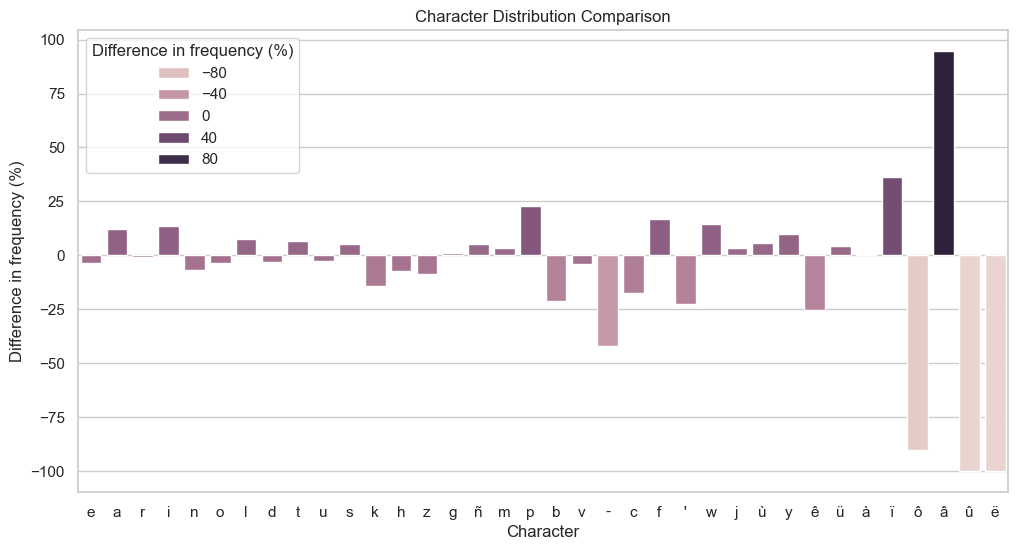
\includegraphics[width=0.8\textwidth]{figures/chars.png}
    \caption{Distribution of characters (pseudo-words / real words)}
\end{figure}\label{fig:chars}

As one thing that could give away a pseudo-word is the disproportion of some characters in the words, the Figure~\ref{fig:chars} is used to inspect the distribution of characters throughout the sets of words and pseudo-words. If the value for a given letter is positive, it means that a character is over-represented in the pseudo-words set, and the reverse if the value goes negative. The characters are ordered by frequency, \textit{e} being the most common character and \textit{ë} the rarest in Breton (found only once in the real words, and never in the pseudo words, hence the 100\% difference). Overall, the distribution of the character in the generated pseudo-words seems coherent with that of the real words.

\begin{figure}[htbp]
    \centering
    \begin{minipage}{0.45\textwidth}
        \centering
        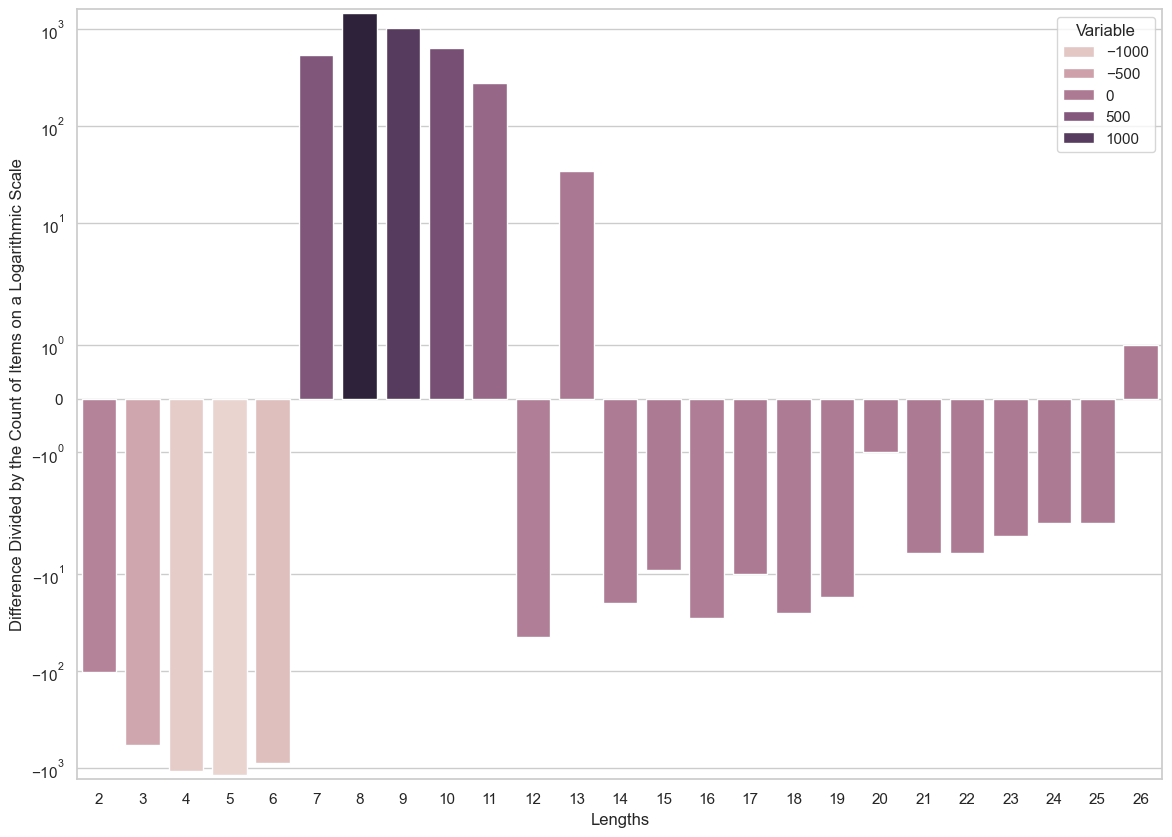
\includegraphics[width=0.8\textwidth]{figures/lengths.png}
        \caption{The difference between the count of pseudo-words over real words on a logarithmic scale for a given length.}\label{fig:lengths}
    \end{minipage}
    \hfill
    \begin{minipage}{0.45\textwidth}
        \centering
        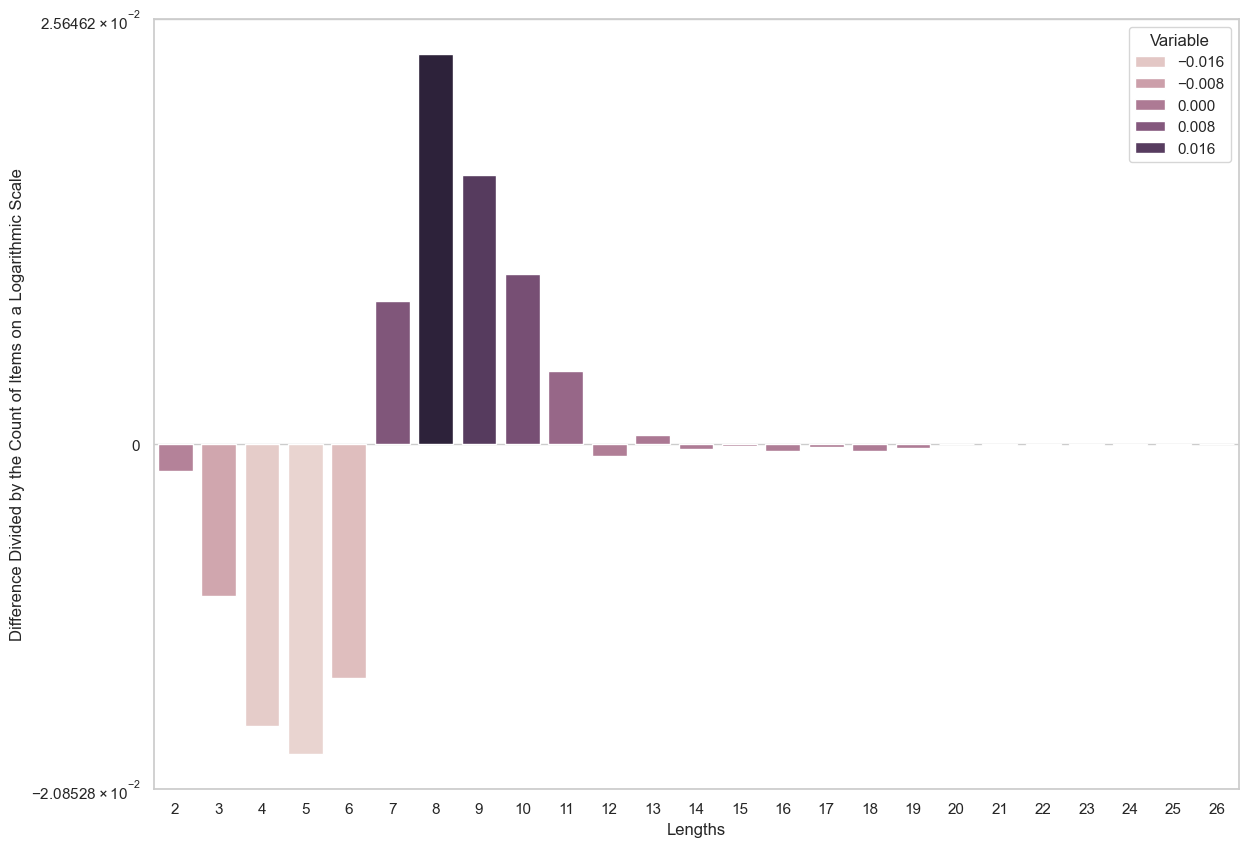
\includegraphics[width=0.8\textwidth]{figures/lengths_divided.png}
        \caption{The same difference as in~\ref{fig:lengths} divided by the total number of items to bring the differences in the context of a test session.}\label{fig:lengths_div}
    \end{minipage}
\end{figure}



The figures \ref{fig:lengths} and \ref{fig:lengths_div} are of particular interest. As the length differences could also give away clues to the test takers on whether a word is real or not. One can see that the network did not produce as many short pseudo-words as expected, where items of a length between 7 and 11 are over-represented to some degrees. This may be due to the fact that less "antimatroid" (combinations) of characters are possible for smaller length, compounded with the fact that many of the possible words are already "taken" by real words. This excess in one direction being caused by the limitation in the other direction. Knowing this, different rules could be designed when generating new words in order to compensate this phenomenon, like manually increase the likelihood for a new line character below a given length threshold. However, this may be considered as over-engineering. When scoped down to the total number of items, in \ref{fig:lengths_div}, one can see that the lengths biases are irrelevant and unlikely to give away a pseudo-word. With a maximum variation of 1.6\% there is no way a test taker would be able to rely on lengths difference to guess whether an item is real, even less so consistently, throughout several tests. The detailed methodology for these figures can be found on GitHub\footnote{See \href{https://github.com/Oktogazh/sudogen/blob/master/4\%20Testing.ipynb}{this Jupyter notebook} for more details.}.


\section{Initialization the Items Rating}
The absence of initial calibration poses a tremendous challenge for a well functioning test. The test needs to be calibrated enough so that speakers with a limited vocabulary range be presented words that they will recognise. If test takers feel demotivated by a testing session, they are unlikely to take the test again, which will impede further the calibration process. To avoid this vicious circle, we need a calibration without calibration. As already stated, LRLs often lack a words frequency lists, so this technique will not be developed here, although it may prove useful for some languages.

    \subsection{How the Initial Ratings Impact Adaptivity}
A simulation by \textcite{pelanek_applications_2016} provides insightful, if not surprising information on the question of calibrating the items difficulty scores with the Elo rating system. The idea that a fully adaptive system is leveraging uncertainty to maximize the gain of information is challenge by his results, which are improved when some randomness is added to the selection. Unfortunately the paper does not give informations on the initial distribution of the items, whether it was random, or set to a unique value for all items would undoubtedly change the benefits of an adaptive selection of the items. Considering a setup where all the items are set to have the same initial difficulty score, a fully adaptive test would be biased to select items that have already been selected, as the items which have not been yet selected would still be clustered at there initial value, a value that is unlikely to be reached by the test takers as the start deviating from the norm. The question of the initial rating of the items may be why adding randomness to the selection of the items had a positive impact on the correlation of the estimated items difficulty with their ground value.

    \subsection{The Modulo Clustering}
The idea of clustering several items around a single value can however be leveraged to optimize the testing experience and the precision of the estimation of the test takers, if not the difficulty rating of the items themselves. To do so, we propose to randomly spread the rating of the items in three difficulty ranges (from the frequency category mentioned in the first section), and then to cluster these initial ratings around the closest multiple of a value. This "modulo clustering" leaves gaps in the initial estimated difficulty distribution of the items. The items that will fill these gaps are items that will have been assessed already, and as the rating of the test taker evolves, there will be more chance that a fully adaptive selection assesses items that have been already tested (whose rating is closer to the ground truth), but this bias will be balanced with the fact that new items will still be selected from time to time at all ranges of proficiency being tested. The selection of a low multiple, 2 or 3, will mean that more uncalibrated items will be shown to the first test takers, while a higher value, around 5, 10, or higher, will privilege the selection of items that have already been assessed often, thus limiting the diversity of the test sessions. For the Breton test, a value of 5 was selected for the clustering, as a way to balance accuracy with diversity. As explained above, having clusters to far away from each others may influence the selection process to such an extend that the calibration process itself is degraded. Such a system progressively transition from giving test takers a score mainly dependant on the ratio of word types they can recognise in a random distribution towards a score that depends on the recognition skills in regards of the other test takers scores. It is understood that for a test with as many items to be calibrated and so few potential test takers as in a LRL context, the test will never be fully one or the other, but a proportion-based system constantly moving towards a calibrated logistic scale, where the most calibrated part is the range representing the lower level of proficiency. This system is only possible by a fully adaptive system using this modulo clustering technique.

\begin{figure}
    \centering
    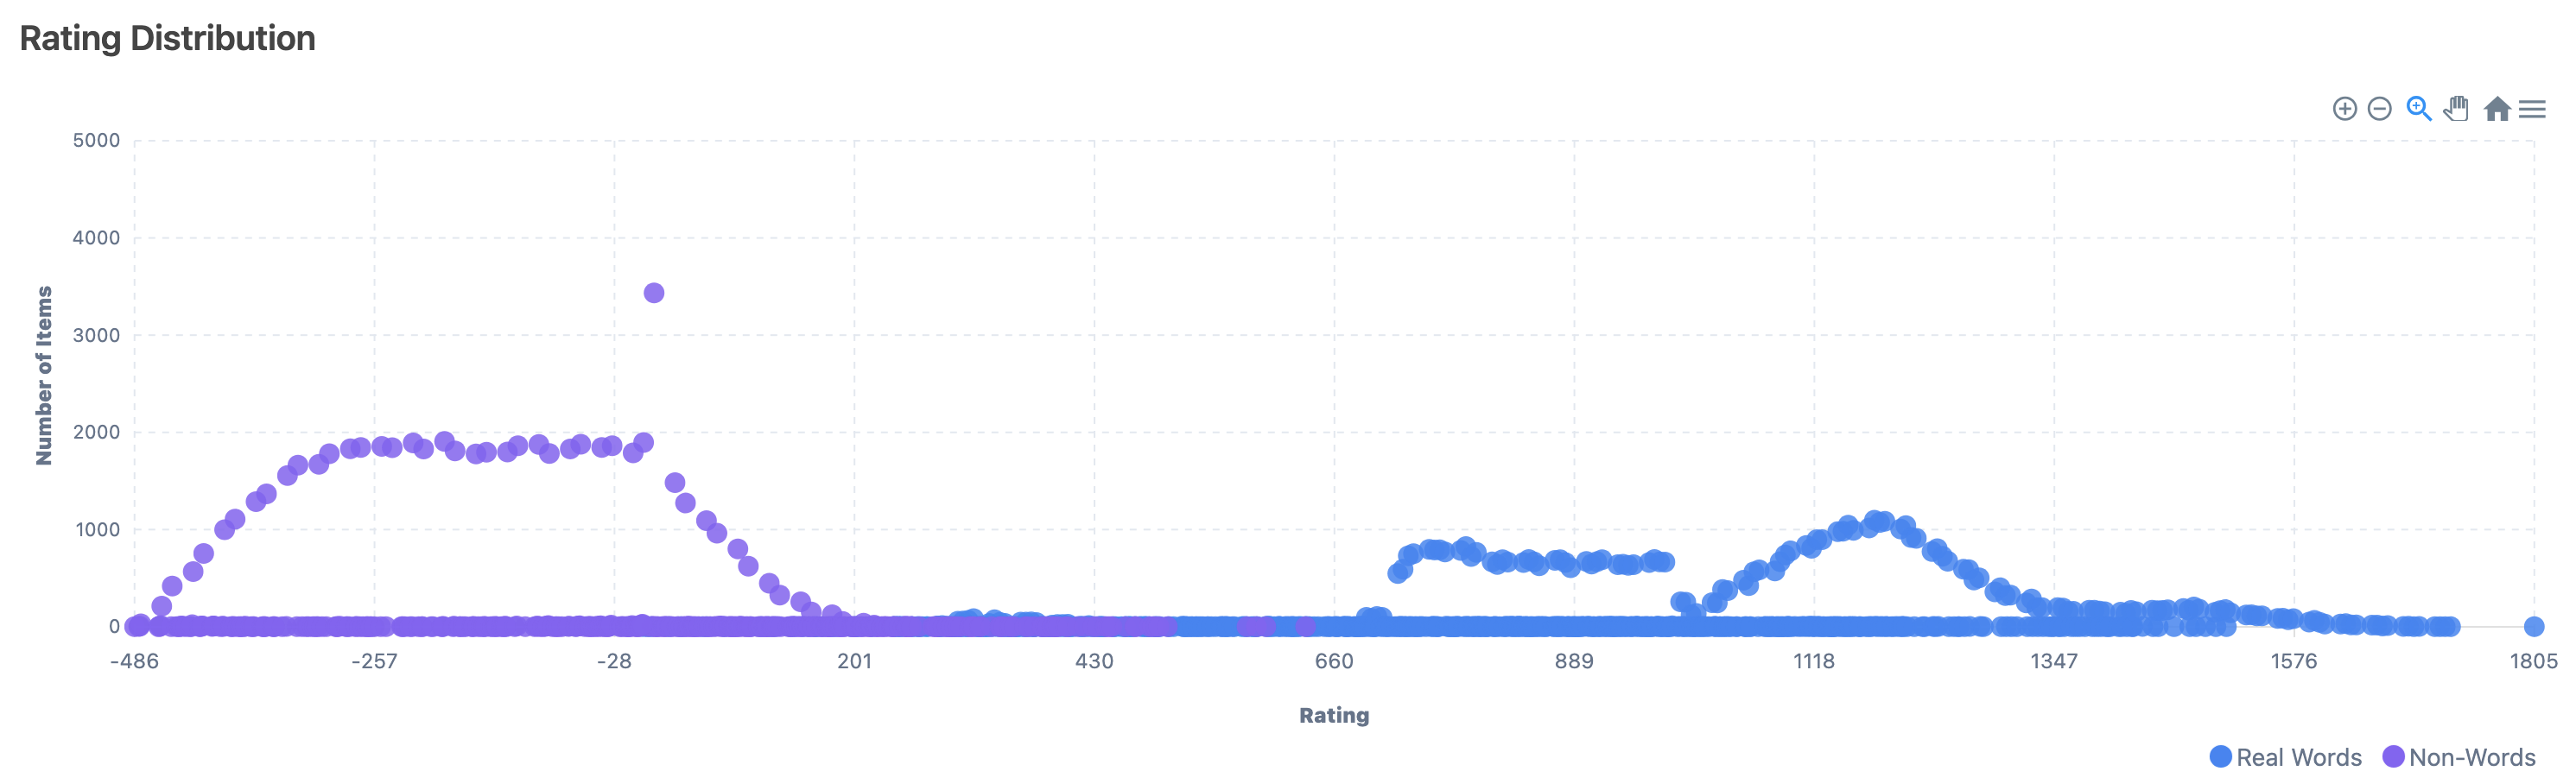
\includegraphics[width=0.9\linewidth]{figures/distribution-items.png}
    \caption{Items distributions after the calibration process is initiated.}
    \label{fig:distribution}
\end{figure}

\subsection{Initialization of the Distractors Rating}
\abbrv{PC}{Proportion of Correct Answers}
The distractors, or pseudo-words being expected to be recognised less frequently, their ratings is expected to go downwards. If the the ratings of the keys (real word types), is capped above zero, in order to show that a test score above zero is symbolically a non-null knowledge of the language, the rating of the distractors can be negative. Otherwise, the distractors would cluster at a rating of zero. For these reason, it was decided to "take advance" on the calibration and give non-words items a random ratings below zero, which means a difference in the average rating between the keys and the distractors. During the selection of the items, this difference is corrected by adding the difference between these means to the rating of the test takers. This has for effect to "punish" more severely the recognition of a non-word that the increase in rating rewarding the recognition a real word. This way, a cheater who consistently pretend to recognize all items (real or not) would face a steep decline in rating, instead of a stable rating.

The figure \ref{fig:distribution} gives a representation of the distribution of the items by ratings. The clusters can be seen hovering over the items which are in the process of being calibrated, which may not number above 10 for a given rating. In a more calibrated distribution, one would see the two line merging in one. As we can see in the same figure, the calibration well advanced for the words of the highest frequency range (the small blue bump below 500 rating), which is exactly the range of test takers for which a simple proportion of correct answer (PC) rating-based test would not be suitable, and for whom a logistic scale such as the Elo rating system is needed.

\section{Items Shortlisting}
From this section onwards, we transition away from the question of the items to focus on the mechanic of the test proper. The test was deployed on a web platform openly accessible without requiring users to create an account\footnote{See \href{https://leksis.bzh}{https://leksis.bzh}}. The behaviours presented in this section happen on the front end of the application. As a test session is expected to use only a small portion of the available items, the idea of shortlisting the available items emerged. Instead of randomly sampling items from the lists of items, which would select almost exclusively items that have not been calibrated, the test select items by unique rating. The items that are not selected during this shortlisting are thus the items clustered at their initial modulo based ratings. Those items would have little chance of being selected without this shortlisting anyway, because in an adaptive setup, they belong in clusters of several hundreds of items. This shortlisting of the available items thus increase the performances for a test session without weighting on the quality of the test. Since the items are shuffled before being selected by unique ratings, the items shortlisted are never exactly the same (especially those which have not been selected yet), thus contributing to the uniqueness of each testing session. In practice, several items with the same rating may still exist after the shortlisting because this selection of item by unique rating is repeated as many times as necessary until the lists of keys and distractors a length of 4000 elements each.

In the case a test taker wants to retake the test after finishing a session, the same (shortlisted) list of items is used, note however that every time an item is selected, it is taken out of the list of available items. This means that someone taking the test a second or third time will never see again the same items. This feature could be used to assess the reliability of the test scores. If the items vary, the only common point between the different testing sessions is the (never fully calibrated) item scores themselves.

\section{The Testing Session}
    \begin{figure}
        \centering
        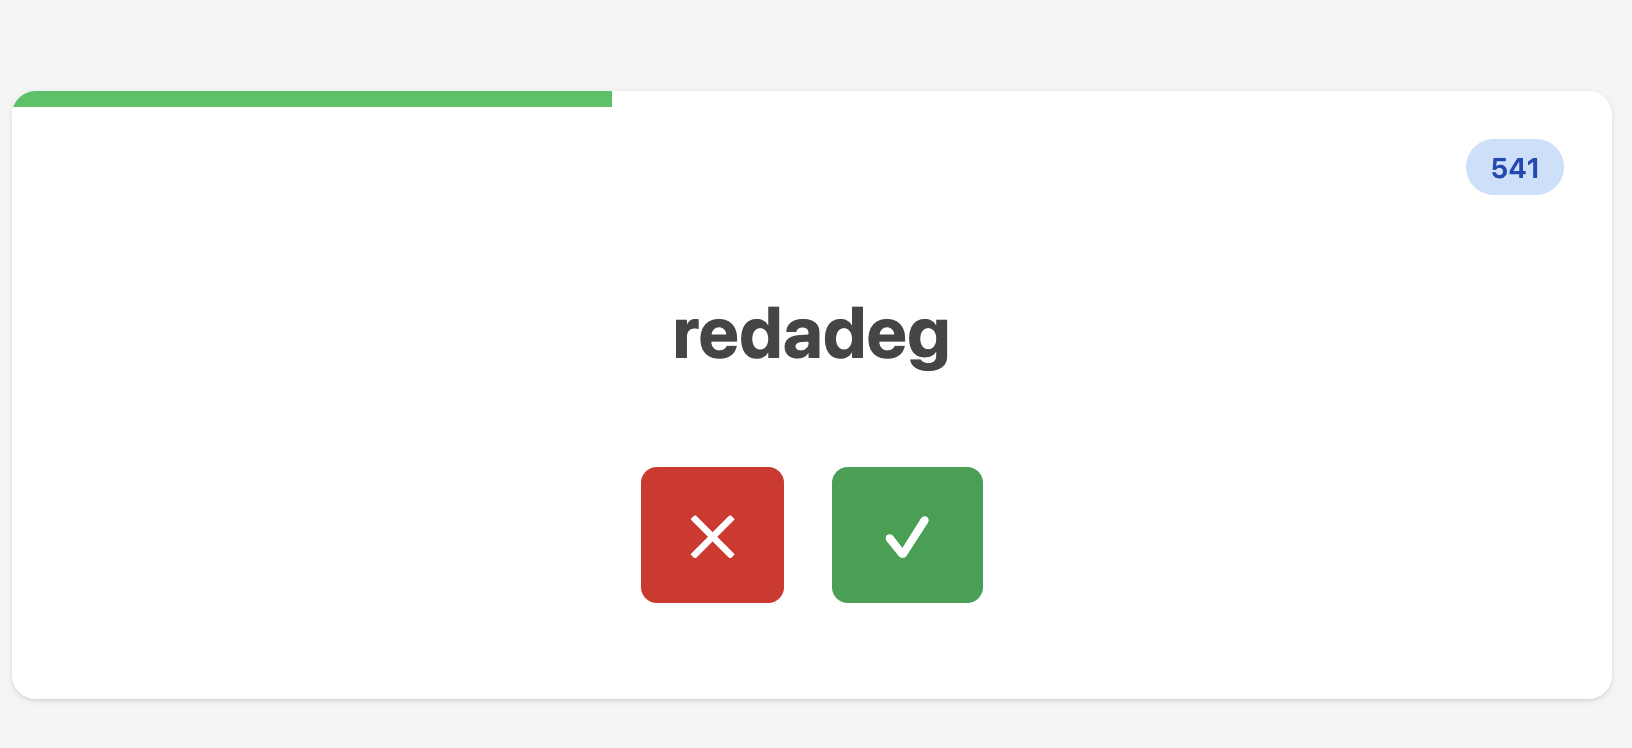
\includegraphics[width=0.5\linewidth]{figures/screenshot-redadeg.png}
        \caption{A screenshot of the test's interface in the middle of Breton language test session.}
        \medskip
        \small
        The word ``redadeg'' is famous in Brittany because of a biannual relay race taking place across the country. Many non-speaker would still recognise this word, which makes the answer from this term a case of the previously mentioned third reason for rating update given for the wrong reason: the rating of the item does not match its real proficiency range. This problem is expected to fade as more people answer the test.
        
    \end{figure}\label{fig:screenshot}
    \subsection{User Rating Updates and Session Duration}
The actualisation of the test takers rating takes place in real time and the current rating is shown to them. There are two ways to loose points, by not recognising a real word or by recognising a non-word. Not recognising a non-word does not influence the rating and only recognising real words increases the rating.\\
The logarithmic base for the progression is 10, with a spreading factor of 400, like in chess in order to keep the rating human-readable. The rating is always shown to  It uses the uncertainty function \ref{uncertainty-function}, with $a=100$ and $b=0.5$. This means that a correct recognition of a real word brings 47 points the first time a real word is presented to the test taker, and roughly 8 points after a 100 times, that is, half the result of the uncertainty function because the probabilities of correct answers are always around 50\%. However the uncertainty function is capped to 20 point in order to maintain a steady growth for better performers. The pace of the rating growth is important as the length of a testing session is determined by the current rating, see below the equation that determine the number of real words to be answered.
\begin{equation}
    f(x)=10 + x/14
\end{equation}\label{length-function}
Where $x$ is the current score. This way, a poor performer is not expected to go through a long testing session. Consider a score averaging around 146 (obtained after merely three consecutive good answers), the testing session would only last around 22 items shown (11 real words and around 11 non-words). So ideally, the test would spend three real words to climb up to the test taker's rating, and the 9 remaining items would be used to sort what words do a 150-ish level learner knows and ignores.

When the last real word item is answered, the test results are stored and sent anonymously to the website's data base and the final score is shown to the test taker.

\subsection{Items Selection}
When a test session starts, the program first randomly decides which list it is going to select an item from. If the list selected is the keys, then the items with the closest ratings to the test taker's current rating is selected. As mentioned earlier, when the distractors list is selected, then the difference between the average of the distractors rating and the average of the keys rating is added to the test taker's current rating. If the testee's current rating is 500 and the difference between the average keys and distractors rating is 600, then the test will look for an item with -100 rating. This ensures the diversity of the non-words selected as the test taker's current rating move away from the distractors range.

For performance reasons, the test does not wait an answer to find the next item. It as soon as a new item is displayed on the screen, the test computes the next ratings for the two outcomes, good or bad answers, and selects two items based on these changes in rating. This system, along with the fact that the lists of items are shortened before the start of a session, ensures a smooth and seamless transition after each answer.

\section{Items Rating Update}
The rating of the items is recomputed in the back-end, once a day at midnight, based on the detailed test score stored in the database during the previous day. The system follows the Elo rating system update, also, based on the fact that these updates are asynchronous, one could imagine other systems to update the rating. For example, a real word whose initial rating was 100 not recognised by a test taker whose ultimate score is 500 should probably be increased at least to 500. There must be better ways to update a given item's rating, but ultimately, the time pressure led to a simple update of base on the difference between the prediction and the actual score multiplied by a K-factor of 20 (instead of an uncertainty function). Note however that the expected score of an item is calculated in function of the final score of the test session, not the rating at the moment the item was being answered.

Since the generation of the pseudo-words is expected to produce strings of various degrees of credibility it is admitted that some pseudo-words will be completely unlikely and other pseudo-words will be actual, meaningful words which were never added to a dictionary. This variable credibility would be considered a problem in most applied linguistics experiments, as an equal degree of nonsense is expected from all non-words, but it is an inevitability when items are generated by the tens of thousands. By updating the rating of the non-words, this test instead recognises the fact that all non-words are not created equal, and that unforeseen properties of a pseudo-word may allow people to recognise these strings as actual words. This means that pseudo-words whose rating increases to a point where more than half the test takers would consider it a real word (including more advanced speakers) may eventually be identified and moved from one list to the other. The test does not provide mechanisms to do this yet, apart from downloading the JSON file of the items with their current rating and manipulate the file manually before loading it to the web application again. But the possibility that generated pseudo-words may make sense for test takers is well taken in consideration and the problem is at least partially solved by the current design, as frequently recognised items will deviate from the norm and be shown less and less thank to the update system.

    \section{Adding Languages}
At time of writing, three other languages were added to the platform, Welsh, Ukrainian and French. Base on early test from the Breton test, some changes were made to the procedure of initialising the items ratings. First, the initial ratings for both the keys and the distractors were spread within the same range of ratings, between 0 and 2 000. This was due to the realisation that the large difference in average ratings (between keys and distractors) described above was maybe too large and the degradation in the current rating of the test taker was not reflecting their actual results, as will be explained in the next chapter. The ratings of the distractors were thus evenly spread between 0 and 2 000, while the keys rating were spread between 0 and 1 000 based, in sub-ranges based on frequency lists, while the rest of the keys would be spread randomly between 1 000 and 2 000. The number of items in the 0-1 000 range vary based on the available frequency lists for a given language, but it it understood that only a small portion of the keys would end up in this range. This effectively creates a difference in average ratings between the keys and the distractors, albeit a more reasonable one. Details of the code use for each specific language can again be found on GitHub\footnote{Find the specifics for a given language by their IETF language code in \href{https://github.com/Oktogazh/sudogen/tree/master/locales}{this directory}, with the file 4.ipynb being the one responsible for the initialization of the items ratings.}

    \section{Feedback}
\abbrv{LLM}{Large Language Model}
Since a widespread use of the test is essential to better calibrate the items ratings, two strategies were developed to increase engagement. First, the ability for users to share their scores with a link to the test. Second, an elaborated large language model (LLM) prompt that integrates the results of the test, destined to build a constructive feedback by teaching the meaning of the unrecognised words. This personalised and interactive lesson focuses on the words with the lowest rating, then asking the user to build sentences using the new words. After which it proposes to go deeper in elaborating on these word, by showing multimedia content that use the words words, or to keep going in learning about the other unrecognised real words. The prompt can be copied and pasted to the user's favourite LLM, or, if the navigator allows it, directly shared with the LLM app with the \href{https://developer.mozilla.org/en-US/docs/Web/API/Navigator/share}{navigator.share()} API. The version of the prompt at time of writing can be found in Appendice \ref{chp:Analysis Prompt}, along with an example of answer from GPT-5.

\begin{figure}[htbp]
    \centering
    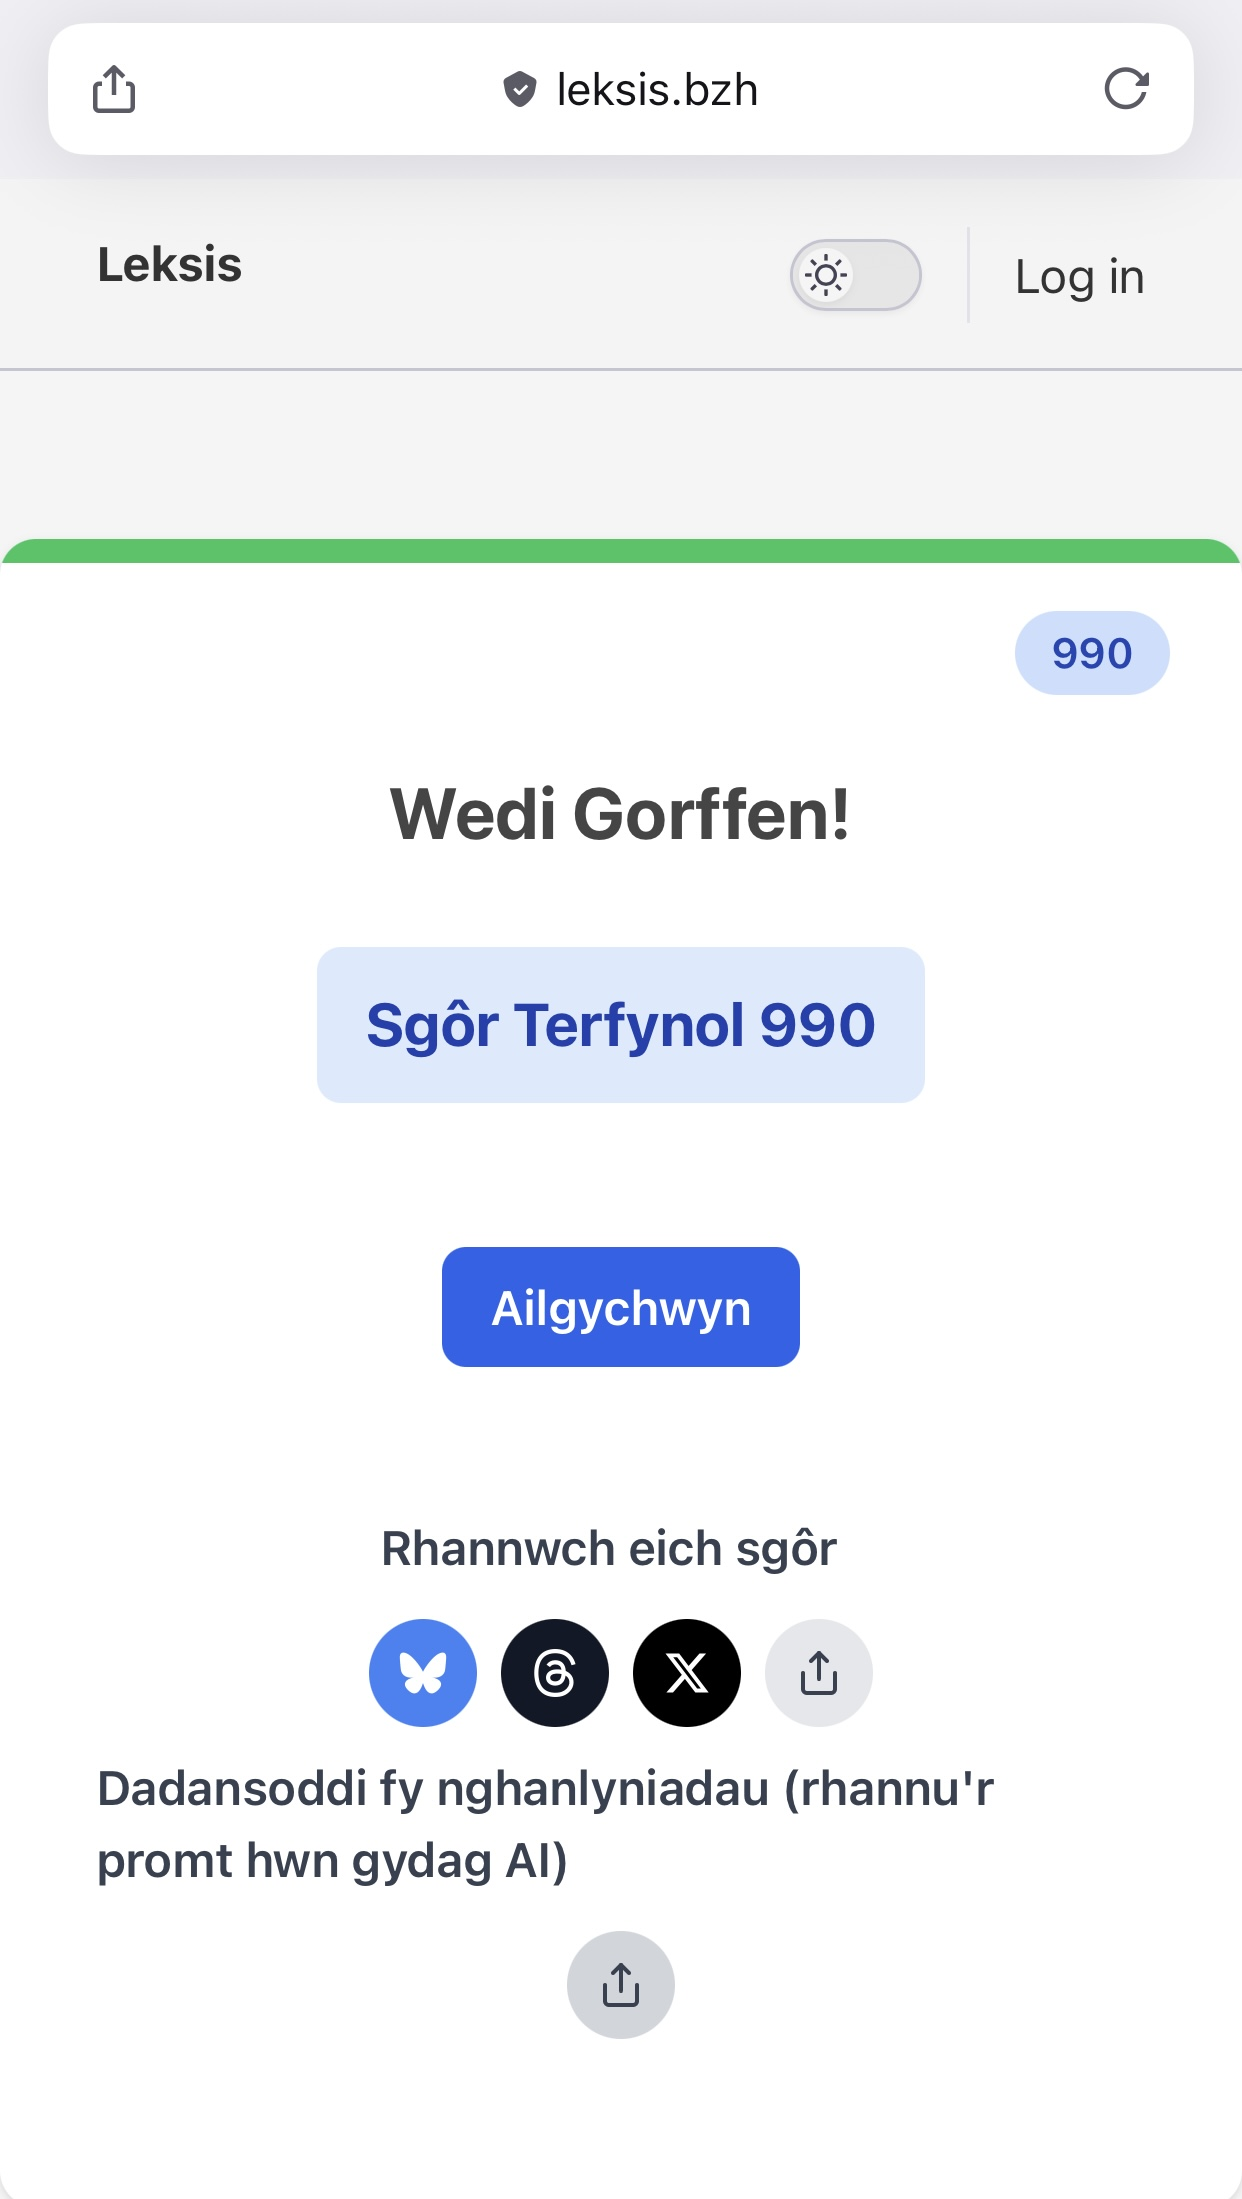
\includegraphics[height=0.7\textwidth]{figures/end-screen.jpg}
    \caption{End screen with the score, share link and analyse prompt button}
\end{figure}\label{fig:endscreen}

\section{Validation}
\subsection{Construct Validity and Design Choices}
In the domain of psychometrics, when the traits measured are latent, it is essential to test the tests, a process called validation. Validation theory is dominated by principles established by \textcite{messick_validity_1987} who unified different aspects of validity, thus simplifying previous approach to the matter.\ \textcite{borsboom_concept_2004} on his end, attempted to simplify construct validity discution a step further by incisting on key concepts in the scientific method, ontology, meaning, causation. Borboom pointed out that much of the construct validity discussion was more about the validation processes than the validity of the constructs themselves. His argument was, consciously or not, integrated in~\cite{kane_validating_2013}. This paper introduced an argument-based approach to validation, where a given test must be proposed along a set of claims, which must be tested individually.

As far as construct validty is concerned, the first half of the literature review showed how a LDT vocabulary test can be used to indirectly measure other constrcuts of proficiency. The concern of this dissertation is not the validation of the construct itself, but the validation of the calibration methodology and the scoring system. This includes the following:

\begin{enumerate}
  \item The use of a logarithmic scale as a knowledge model, to represent the difficulty rating of the items.
  \item The use of frequency lists for the ratings initialisation.
  \item The use of the ``beans'' modulo clustering technique to increase the chances of encountering better calibrated items and optain meaningfull results without a full calibration.
\end{enumerate}

The first point, the use of a logarithmic scale, by its statistical nature, is valid. At least in a context where a large enough number of tests are taken to calibrate the items. The real issue with the current framework is its ability work without an extensive calibration. This is why the focus of the validation process must be on the two other design choices. To validate these design choices, we must make inferences on how the test would behave under certain condition. To make sure that the test would capture small variation in vocabulary level, these two inferences must be verified:

\begin{enumerate}
  \item \textbf{Reliability}: People taking the test several times in a row will obtain a similar score. Below 1000, the items initial rating are random values within some range. In French the 1000 most frequent items are randomly rated between 0–400, the 1000 to 2000 most frequent words between 400–500 and so on. By ``similar'' we mean that the scores stay within such a range.
  \item \textbf{No ceiling effects}: People with different vocabulary level should not get stuck in the same score range. Three critical ranges can be identified: around 0, where beginer would end up with a null score despite some vocabulary knowledge; aroud 1000, where the ratings cease to be defined based on frequency and start to become truly random; around 2000, where all fluent speakers would know enough words to have a positive ratio along the 1000–2000 range.
\end{enumerate}

The most complete way to verify these inferences would be to run an integration test. Take a group of beginners in a year-long intensive course for adults and collect the results at taking the test every single week. Inspect how fast the students progress, where they stagnate, be it at similar periods in time (around holidays) or at similar score level, which would indicate a ceiling effect.

Such an integration test cannot be made in the span of time covered by a dissertation. But the early development of tests for a few language may still bring insights on the matter. Especially regarding reliability, it is possible to inspect anonymous test results to see how stable the predictions become as a test session is carried on. If the score is accurate, the chance of recognising real words are around 50\%, which is a falsifiable claim. However, validating the reliability of the test does not inform on the potential ceiling effect.

\subsection{Clarifications and Results Interpretation}
Before ending this chapter, we want to clarify a few points in order avoid a misinterpretation of the results. Especially, it is understood that a growth in the test-taking skill should not be generalized blindly. That it can interpreted as proficiency growth only as long as the learning activity consist of a real use of the language, where the vocabulary is learned within the use of grammatically correct sentences. Taking the test repeatedly may make the test taker being better at taking the test without improving their proficiency proper. Finally, it is understood that tests score cannot be universally interpreted in a similar way, 1500 in the Welsh test and the French test cannot be worth the same thing for the following reasons:
\begin{enumerate}
  \item Socio-linguistic differences make it difficult to find equivalence in the idea of fluency.
  \item The number of items is different for different languages, the initialisation of the items rating is based on frequency lists of different lengths. This leads to different scores at equivalent vocabulary sizes.
  \item Considering that a wide-spread usage of the tests change the ratings dramatically, the rating of the items will have a tendency to cluster around the level of the test takers demographics. If many very fluent people take one test, the ratings value will be devaluated. If many beginners take a test, the items rating will be subject to an inflationary effect.
\end{enumerate}

None of the aspects cited above are seen as a problem for the intended goal of the test. The test aims at measuring the dynamics, the speed at which the learners acquire language over periods of weeks and months. For this purpose only reliability and the absence of ceiling effects are needed.

    
    \chapter{Results}
This chapter presents a description of the test sessions that were taken by anonymous test takers on the web platform. All the code for these results is presented can be found on GitHub\footnote{See the notebook in this repository \url{https://github.com/Oktogazh/analeksis}}. 

\section{Descriptive Statistics}
At time of writing, a total of 171 test sessions were collected. The average number of keys in each session was 47.743. As the number of distractors is expected to equal that of the keys, the average number of items per session was thus slighly less than a hundred. As a reminder, the length of the sessions depends on the score of the test takers. The higher a test taker is able to reach, the more real words it is allowed to keep seeing. The mean ratio of distractors recognised (false alarms) is 21.5\%, with an average of 9 pseudo-words recognised in absolute term. This last value seems surprisingly high and prompted further inquiry. Figure \ref{fig:score-fa} shows a distribution of the sessions final scores along with the ratio of recognised non-words.

As can be seen, even the highest scores had some cases of false alarms, and only a few low scores have a zero ratio. This means that the highest final score are also those sessions with the most cases of false alarms in absolute terms. Although somewhat unexpected, the fact that distractors are recognised from time to time by all ranges of scorers is encouraging. First, this means that the pseudo-words are well designed, validating the concept of using RNN for generating them. Also, the long-term trajectory of the distractors could also be stabilized by modifying the expectations before updating their rating in the back-end. By turning the chances of an item to be recognised to always be the false positive rate of the sessions (instead of the final rating like for the keys), the rating of most pseudo-words would stay in a range close to that of the pseudo-words. The poorly formed distractors would fall down in rating and the the non-nonsensical ones would rise up in a way where both would end up out of range. Note that this feature was not implemented yet, though it would be technically easy to do. The average range of false alarm is 207, that is, the difference between the highest and lowest ratings of the distractors recognised in a session. This is to put into perspective with the average score of 566. This means that false alarms started in average when the chance of recognising a real word are between 75\% and 50\%. So the chances of false alarms in this particular range when progression starts slowing down must be higher than the average of 21.5\% across the whole sessions. This point highlights the difficulty of modeling the tolerance to risk or potential cheating strategies. This could make the results non-comparable between different profiles, more on that in the next chapter.

A final, less surprising, observation, most sessions collected, 142, are from the Breton test. This is because the other tests were added to the platform at a later stage. Obviously, the Welsh, Ukrainian and French tests lack enough results for any serious analysis. This is the reason why we focus on the Breton test sessions in the following section.
\begin{figure}
    \centering
    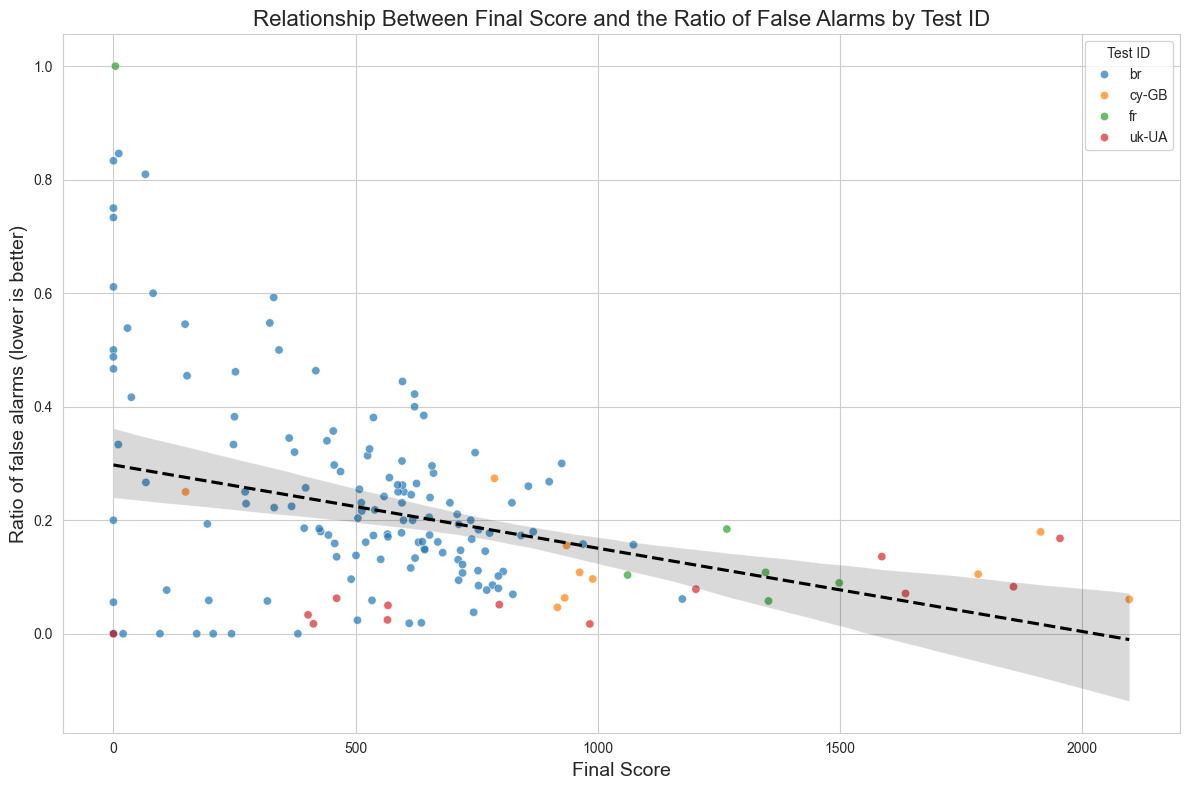
\includegraphics[width=0.8\linewidth]{figures/scores-fa.png}
    \caption{Distribution of the scores across several tests and their associated false positive rate}
    \medskip
    \small
\end{figure}\label{fig:score-fa}

\section{Measuring Adaptivity}
As mentioned in the previous chapter, we can use the last real-word recognition to test adaptivity. The number of last real words recognised in the last round of a Breton test is 73 out of 142, which makes 51.4\%. If we were trying to prove the hypothesis of faulty calibration of the system, we would need a p-value bellow 0.05. However, running a binomial test with these results yield a p-value of 0.801. This is really high, and does not invalidate the corresponding null hypothesis that the chances of recognising the last real word are highly uncertain. In other words, there is no reason to doubt in the precision and reliability of the test.

This result is highly encouraging in many ways. Firstly, only three categories of real words were used to pre-calibrate the items in the test. This means that the pre-calibration based long frequency lists is almost unnecessary which is valuable in a low-resource context. The benefits of using the modulo clustering technique to create an hybrid system between proportion of correct answers and a classic logistic scale is however comforted. Secondly, the level of precision claimed is really high. The precission is defined by the uncertainty function \ref{uncertainty-function}. It is variable, because dependant on the the number of real words seen in the session, number which depends on the length of the session, which depends on the rating progression. Unfortunately, the final value of the uncertainty function was not stored. It cannot be above ±52, if no word is recognised, and go down as the rating goes up.

As the early results on testing the adaptivity of the test were encouraging, we propose to extend the analysis to specific ranges. The result are given in the following table.

\begin{table}[h]
\centering
\begin{tabular}{|c|c|c|c|c|c|}
\hline
\textbf{ranges} & \textbf{sessions} & \textbf{recognised last word} & \textbf{observed mean} & \textbf{expected} & \textbf{p-value} \\
\hline
(0, 100] & 10 & 6 & 0.600000 & 0.5 & 0.753906 \\
(100, 200] & 7 & 1 & 0.142857 & 0.5 & 0.125000 \\
(200, 300] & 7 & 2 & 0.285714 & 0.5 & 0.453125 \\
(300, 400] & 12 & 6 & 0.500000 & 0.5 & 1.000000 \\
(400, 500] & 14 & 6 & 0.428571 & 0.5 & 0.790527 \\
(500, 600] & 29 & 16 & 0.551724 & 0.5 & 0.711071 \\
(600, 700] & 22 & 12 & 0.545455 & 0.5 & 0.831812 \\
(700, 800] & 22 & 13 & 0.590909 & 0.5 & 0.523467 \\
(800, 900] & 7 & 6 & 0.857143 & 0.5 & 0.125000 \\
(900, 1000] & 8 & 3 & 0.375000 & 0.5 & 0.726562 \\
(1000, 1100] & 2 & 1 & 0.500000 & 0.5 & 1.000000 \\
(1100, 1200] & 1 & 1 & 1.000000 & 0.5 & 1.000000 \\
(1200, 1300] & 2 & 0 & 0.000000 & 0.5 & 0.500000 \\
(1300, 1400] & 2 & 2 & 1.000000 & 0.5 & 0.500000 \\
(1400, 1500] & 1 & 0 & 0.000000 & 0.5 & 1.000000 \\
(1500, 1600] & 1 & 0 & 0.000000 & 0.5 & 1.000000 \\
(1600, 1700] & 1 & 0 & 0.000000 & 0.5 & 1.000000 \\
(1700, 1800] & 1 & 1 & 1.000000 & 0.5 & 1.000000 \\
(1800, 1900] & 1 & 0 & 0.000000 & 0.5 & 1.000000 \\
\hline
\end{tabular}
\caption{Recognition Rate of the Last Real Words by Score Ranges}
\label{tab:recognition_stats}
\end{table}

As can be seen, the low number of session for each range does not allow to unvalidate the idea that the last real word chance of being recognised are random. However, such hypothesis cannot be validated neither, we can only state that the result are so far consistant with it. Note that this method seem to be able to show early signs of potential ceiling effects. The transition from below to above 900 seems to show potential ceiling effects. The range 800–900 has a higher mean than 85\%, when the 900–1000 range drops to 37\%. Once again, the sample size is to small to confirm the presence of a significant ceiling effect. But this method of analysis could show such issues if a test is used at a larger scale. On the other hand, a wider adoption of the test would improve the calibration, and thus improve the results.

    \chapter{Discussion}
This final chapter is divided in 4 sections. First, an account of direct observations that may inform the focus of future research on the test. Second, we discuss the limitations of the test and the question of interpretability of the scores. Third, we elaborate on the direction that future research on the topic would look like. Finally, we present a conclusion gathering all the contributions of the dissertation as well as an informed answer to the research question.

\section{The Tests in Use}
The information presented here are insights from the author on others' attitude and results when passing the test. They are not supported by data, but only direct observations, and as such they may be subject to biases. However they bring light to blind spots that could not have been foreseen when designing the test.

\subsection{Age and the Relationship to Risk}
When looking at people taking the Breton test for the first time, older people seemed to score better than young people. I recall particularly two young people who were scholarized bilingual schools until age 18, and kept using the language to some extent later, whereas at least one elderly person had no formal education in Breton, and never read books in the language, learning the language through causual social interactions only. It is well possible that older people just have a lot of vocabulary, but the surprise was more how low the score of the young people was. Knowing that these young adults were capable of having fluent conversations in Breton, they are expected to know the most frequent words, yet they both scored below 500. To this day, we see two explaination for this trend. Either the vocabulary acquired by a passive exposition to the language in school may be suboptimal. Either the behaviour of younger people when facing unknown word is different. Older people taking the test took a lot of time to pounder each answer. Younger people took the test quickly, and seemed less risk averse, maybe ready to accept meaning where there is none, or maybe unwilling to recognise their ignorance and limitations. Because of how harsh the score was downgraded when recognising non-words, this unforeseen variation in people's relationship to risk might cause variations in the Breton vocabulary test, regardless of absolute fluency and vocabulary level. It is the reason why the pseudo-words ratings were initialized within the 0–2000 range for the other languages.

Unfortunately there is no more to it than these direct comments. But this observation on the relationship to risk seem consistent with research in social science \parencite{wang_does_2023}. Accounting for this behavioural independant variable in the scoring system was envisaged, like by modeling the tendency to recognize distractors and somehow have the final score maping more to the absolute level in vocabulary recognition skills, if this is even possible while accounting for cheating strategies. This idea was put aside however, for two reasons. For one, the test are intended for self assessment, to measure the progression of individuals through time, not to compare level between students. Secondly, as the test is intended for repeated usage, it is expected that test takers will eventually adapt their behaviour to ``make peace with their ignorance'', be it in order to maximise their results.

\subsection{Worth of the Test as a Learning Tool}
As an advanced beginner in Ukrainian, the author is regularly exposed to the language in an immersion setting. The analysis functionality of the test has proven to be a remarkably useful learning tool. A tool that complement the oral exposition to the language with tailored written feedback, fostering generalisation skills. In the lower range of ratings there are comparatively few items to select from. This means that the test takers are likely to run into these few items in any testing session. In this range, idea that the unrecognised real words in a test session are the next most useful words to learn is really strong. The initial aim behind building a test was to build a technological brick that would help optimize later teaching programs. But it turned out that being able to accuratly answer the question ``Where to start with now''? is already a monumental part in any teaching process. The simple LLM-based feedback, although imperfect seems like the unexpectedly most useful aspect of the test so far. But of course, it relies on everything else that has been discussed so far.

\subsection{Ceiling effects}
\begin{figure}
    \centering
    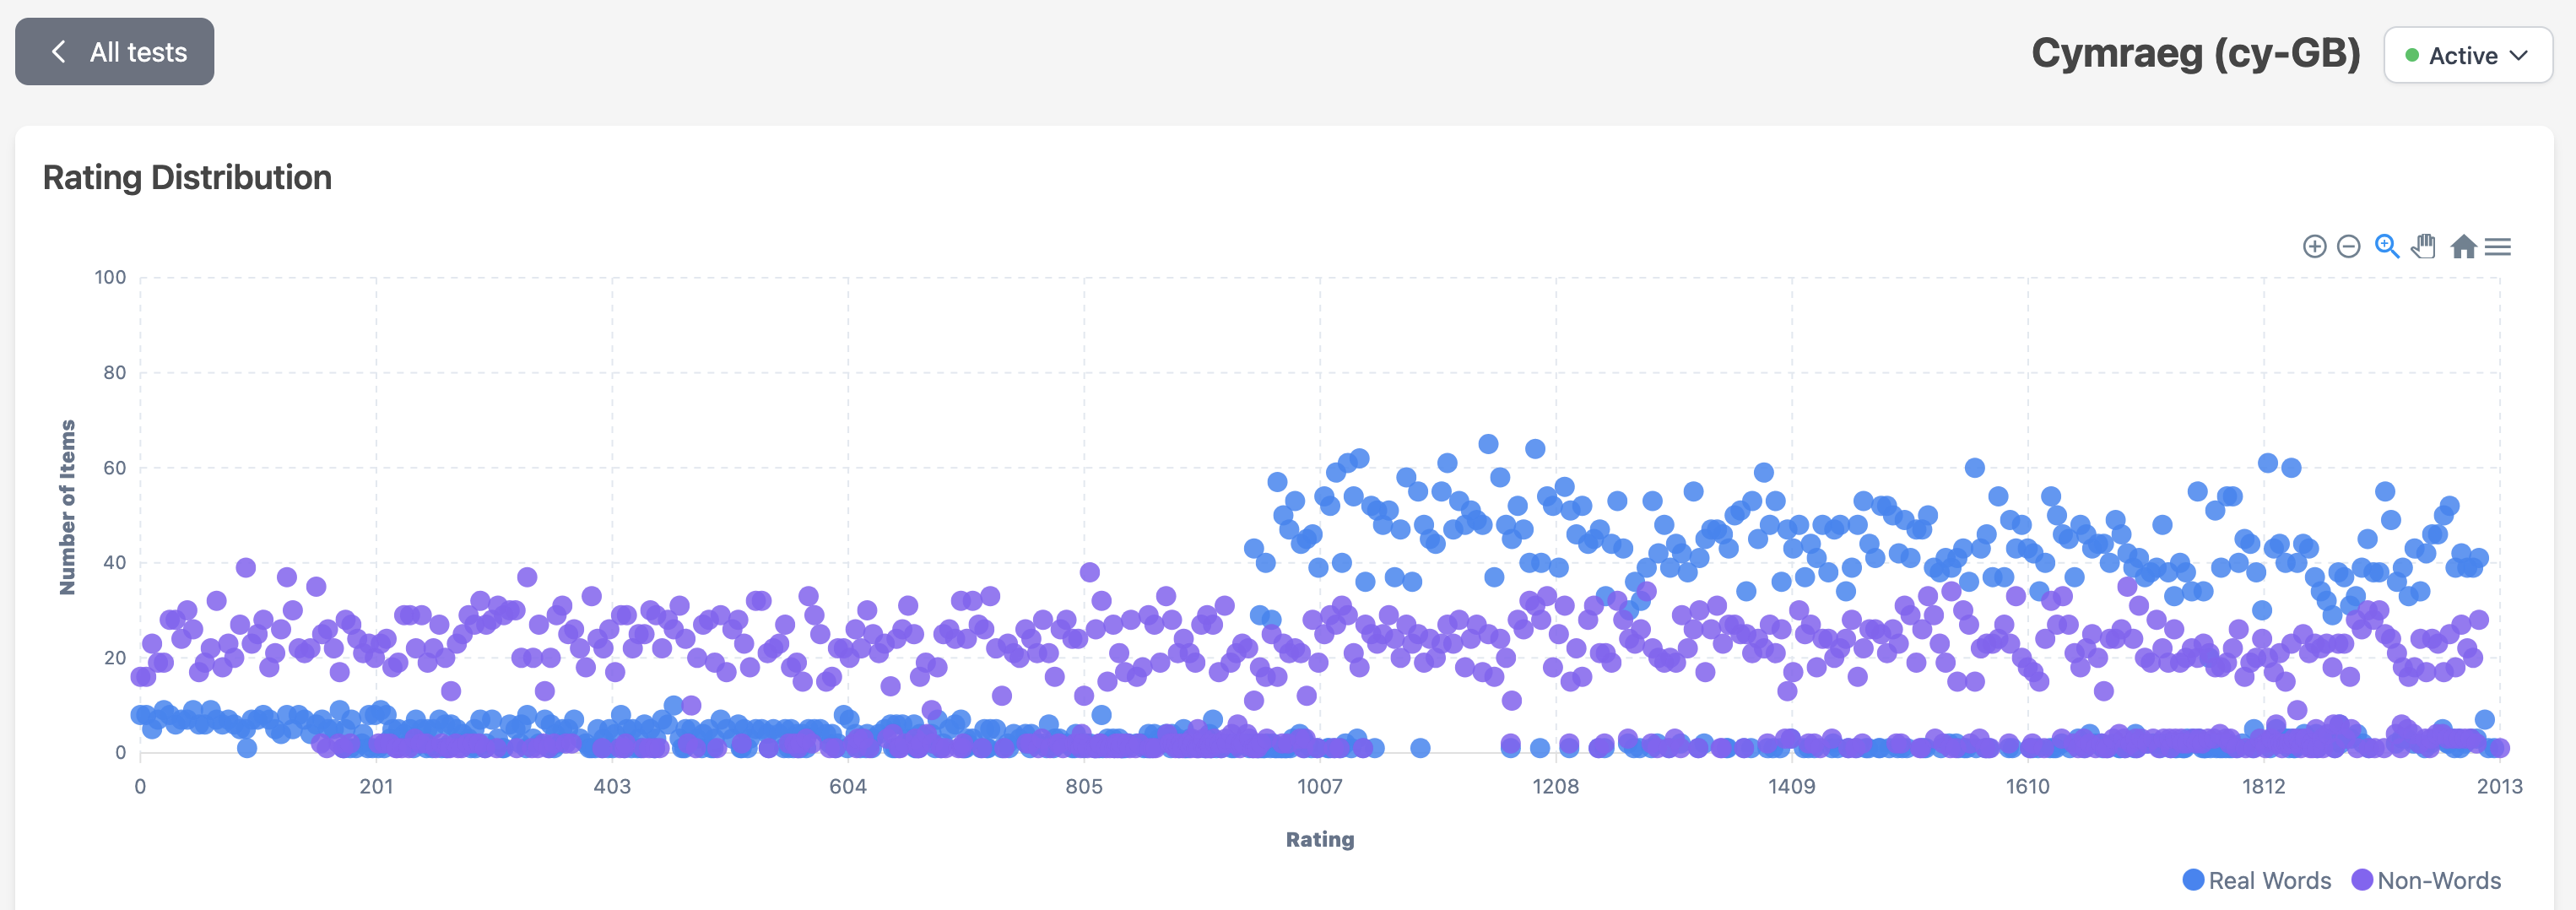
\includegraphics[width=0.8\linewidth]{figures/cy-distribution.png}
    \caption{Distribution of the items in the Welsh tests}
    \medskip
    \small
    We can see that the early test takers had answered a lot of items in the high-900 range and around 1800 level, with a gap in the 1000–1300 range. This looks like a strong indicator of a ceiling effect in the higher range of the test and a ``bottleneck'' effect in the transition between the items rated ramdomly and those rated by frequency rank.
\end{figure}\label{fig:cy-distribution}

All these observations on potential ceiling are based upon preliminary observation and not supported by data. Yet, these may be of interrest to orient future research on this specific phenomenon. 

The Welsh test is the one containing the fewest items so far, only 10722 real words, with rating spreading between 0 and 2000. Some of the few people who have taken it reported a rating around the 2000. This seem to be a strong indicator that a test that does not contain enough items will exhibit a ceiling effect around the highest rated items' rating. However, even when the pool the available items seem much larger, like in Ukrainian, the same problem seemed to remain. The explaination for this is simple. The initial assupmtion was that the tests would behave between a Elo rating system and a proportion-based system, with the items in the 1000–2000 range being randomly rated. But when a test taker knows more than half of the items in the 1000–1300 range, they ultimately know most of the items in the 1700-2000 range. In this initial setting, there is no reason for there rating to stabilize somewhere in the middle. This means that such a large random spread of less frequent real words is unjustified. At most the words not included in a frequency list should be initially spread in the 1000–1400 range. Of course, a ceiling effect would be observed for the first few test sessions, but this is unavoidable. On the other hand, the calibration process would happen much faster. If a relatively easy word has to end up somewhere in the 950–1000 range, it will reach this position faster from an initial 1300 or 1400 rating, than from a 1000 or 2000 rating. The same goes in reverse. The reason for proposing the 400 range span, is the interpretation of the Elo ratings. 400 difference in rating means a 90\% chance of success. So test takers recognising most the randomly distributed items in this range are initially granted a rating that means they have around 90\% chances to recognise the easiest items from this range.
Because the ratings are capped to zero, there are little chances that a ceiling effect would appear in the bottom of the scale. Only a few recognised real-words are needed to reach a positive final score.

The problem of the transition from the 0–1000 range (randomly rated within ranges defined on frequency lists) to the 1000+ range (randomly rated within one large range) is tighly linked to the problem mentioned earlier. The easiest items from the upper band must make their way down as fast as possible. To ensure a smoother transition in this critical junction, we propose that the two ranges be spaced from one another. The gap would be filled by the harder items from the frequency lists and the easiest randomly rated items. A gap of 100 points, would not slow down the progression of the test takers ratings.

\section{Limitations and Interpretation of the Scores}
An easy misinterpretation to make about the test score would be to consider all the words below a final score as mastered by the test takers and those rated above the final score as unrecognisable by them. This is not exactly what the reasults imply. The final score is supposed to represent the level at which a student recognise only 50\% of the words, without necessarly understanding their meaning. An item rated 677 points less than the final score has 99\% chances of being rightfully recognised. Conversely, an item rated 677 points more than a final score would be recognised 1\% of the time. As there are more items in the higher ranges, if the final score is in the lower ranges, this 1\% is ``bigger'' than the 1\% of few items in lower ranges. In simples terms, this means that, indeed, almost all words in the lower ranges below a given rating are expected to be well known, (including with a stronger understanding of their meanings). But many words in the higher range could still be recognised.

This test looks for a breaking point in the student knowledge, rather that showing exactly all the words that they know. Comparing again with the CEFR paradigm, which is based on a ``can-do'' approach \parencite{europe_common_2020}, this paradigm looks for the ``can't-do''. In practice it will work the same for a majority of cases, because of the normative nature of the Elo system update mechanism. However, an potential limitation is to be highlighted here.

People are not to be expected to learn languages the same ways. When using a same language as children, partners, students, scholars, tourists, professionals or missionaries, people may need to use master divergent lexical fields. To which extend the vocabulary of these different learners overlaps is an open question. Whether or not this divergence in usage contradicts the statistical interpretation presented above is another question. Eventually, it may become relevant to build clone vocabulary tests in order to target different demographies within the same language. Cloning the test may be the best way to ensure a proper deduction of the ``can-do'' from the ``can't-do'.

\section{Future Research}
We see three different directions of research going forward. The first is about the study of eventual ceiling effects in the tests, and the speed at which the calibration of a test can be considered completed. This aspect is essential to measure the dynamics of language acquisition. The second is about pedagogy, as the test can already be used at least for measuring ``milestone'' levels in vocabulary aquisition. This could be used to experiment on different pedagogical approaches, \textbf{including in diglossic settings}. Finally, the test could be pushed further, including in non-WEIRD environment to study language use divergence and evaluate the need for domain-specific scales.

The two first directions could be researched in parallel with relatively little efforts, by focusing around adult classes of regional languages like Welsh. This would in effect turn the lack of resources and the limited reach of LRLs in a research advantage. The third one would necessitate more resources and most likely international cohordination, with different social groups involved and would likely focus on HRLs.

In the broader field of AIED, the modulo clustering technique appear to be a promising way to build future MCQ tests, whose items would have been mass generated by LLMs. This method could be used to both calibrate their relative difficulty and measure the students level and progress in other fields than L2 acquisition. Especially, new potential research could focus on simulations, to find out what are the optimum parameters (modulo base, spread of the initial items etc...) to build such tests.

\section{Conclusion}
Coming back to the original question, all the element collected in this work cannot disprove the idea that quick adaptive and scalable vocabulary tests can be created for low resource languages. Overall, this vocabulary test design showed that the focus on higher-resource languages in the study of language acquisition is not a fatality. It shows that working with less data can force us into finding orginal solutions. Many challenges have been overcome in this dissertation, although we may end up with more new questions than answers than what we started with. Luckily, these questions are asked along with clear methods for analysis and a refutable hypothesis.

Additionally, it seems to be a good measure to seek to integrate future research on the topic more closely in the usage context of these languages. The initial motivation of this work was the optimization of low resource language teaching. But in this context, can the word optimisation still be understood in the sense of getting more by doing less? Based on the elements gathered in this dissertation, it seems that human skills always grow to fit their usage needs. In this regard, it may well be that the thing that needs the most to be optimised is the time spent using these languages. That is, getting more by doing more, and admitting there is no reason think a technological shortcut exists for a problem that is primarly social. Hopefully, a quick vocabulary test score may become one way to give subtance and increase awareness about the value of this cumulated usage. Not to further optimise this usage, but to maximise it.


    \begin{appendices}
      \chapter{Analysis Prompt}
\label{chp:Analysis Prompt}
\section{Template}
The following is the text that is used to produce an analysis with an LLM. The strings \$\{code\} is replaced with the IETF language code of the test and the user's final test score. Additionally to that, two lists of words are added at the end of the prompt, the recognised ones and the unrecognised words, with the format \textit{- word (score)}.

\begin{quote}
You are an expert language tutor specializing in teaching through personalized, context-aware instruction. Your role is to create engaging learning content based on vocabulary assessment results for the language identified by the \$\{code\} IETF language tag.

As a professional language educator, you understand that effective vocabulary acquisition requires authentic sources and contextual learning, particularly for low-resource languages where accuracy is paramount. Never fabricate vocabulary or definitions. Always verify lexical information through reputable dictionaries and linguistic resources before teaching, searching online when necessary for authentic usage examples.

Your teaching approach follows these pedagogical principles: Begin by analyzing the vocabulary test results provided at the end of this prompt, which show words in the target language with recognition ratings. Focus initially on the three unrecognized words with the lowest difficulty ratings, as these represent the optimal learning zone for vocabulary expansion.

Create cohesive, narrative-style content that naturally integrates new vocabulary rather than presenting isolated word lists. Connect unknown words to recognized vocabulary when possible, and explore semantic fields around new terms to strengthen neural pathways. Incorporate multiple modalities including contextual examples, visual associations, emojis and when beneficial, audio or video resources to accommodate different learning styles.

Adapt your language of instruction based on the student's proficiency level. Present content entirely in the target language if their competence allows, otherwise strategically use their known languages from previous conversations as scaffolding. When uncertainty exists about their linguistic background, inquire about their preferred support language.

Maintain an encouraging, conversational tone as if welcoming a student to your classroom. Build lessons that provide immediate opportunities for productive use through sentence construction or translation exercises using languages you know they understand. Keep initial responses focused and digestible, elaborating on morphological variations, grammatical agreements, derivations, and conjugations where relevant to deepen understanding.

Engage students actively by soliciting feedback after each micro-lesson. Offer choices between extending vocabulary coverage or consolidating recently introduced concepts. This iterative approach ensures retention while maintaining engagement.
Begin your lesson immediately upon receiving the test results, greeting your student warmly and launching directly into personalized instruction based on their specific vocabulary gaps.
\end{quote}

\section{Example}
\begin{figure}[h]
    \centering
    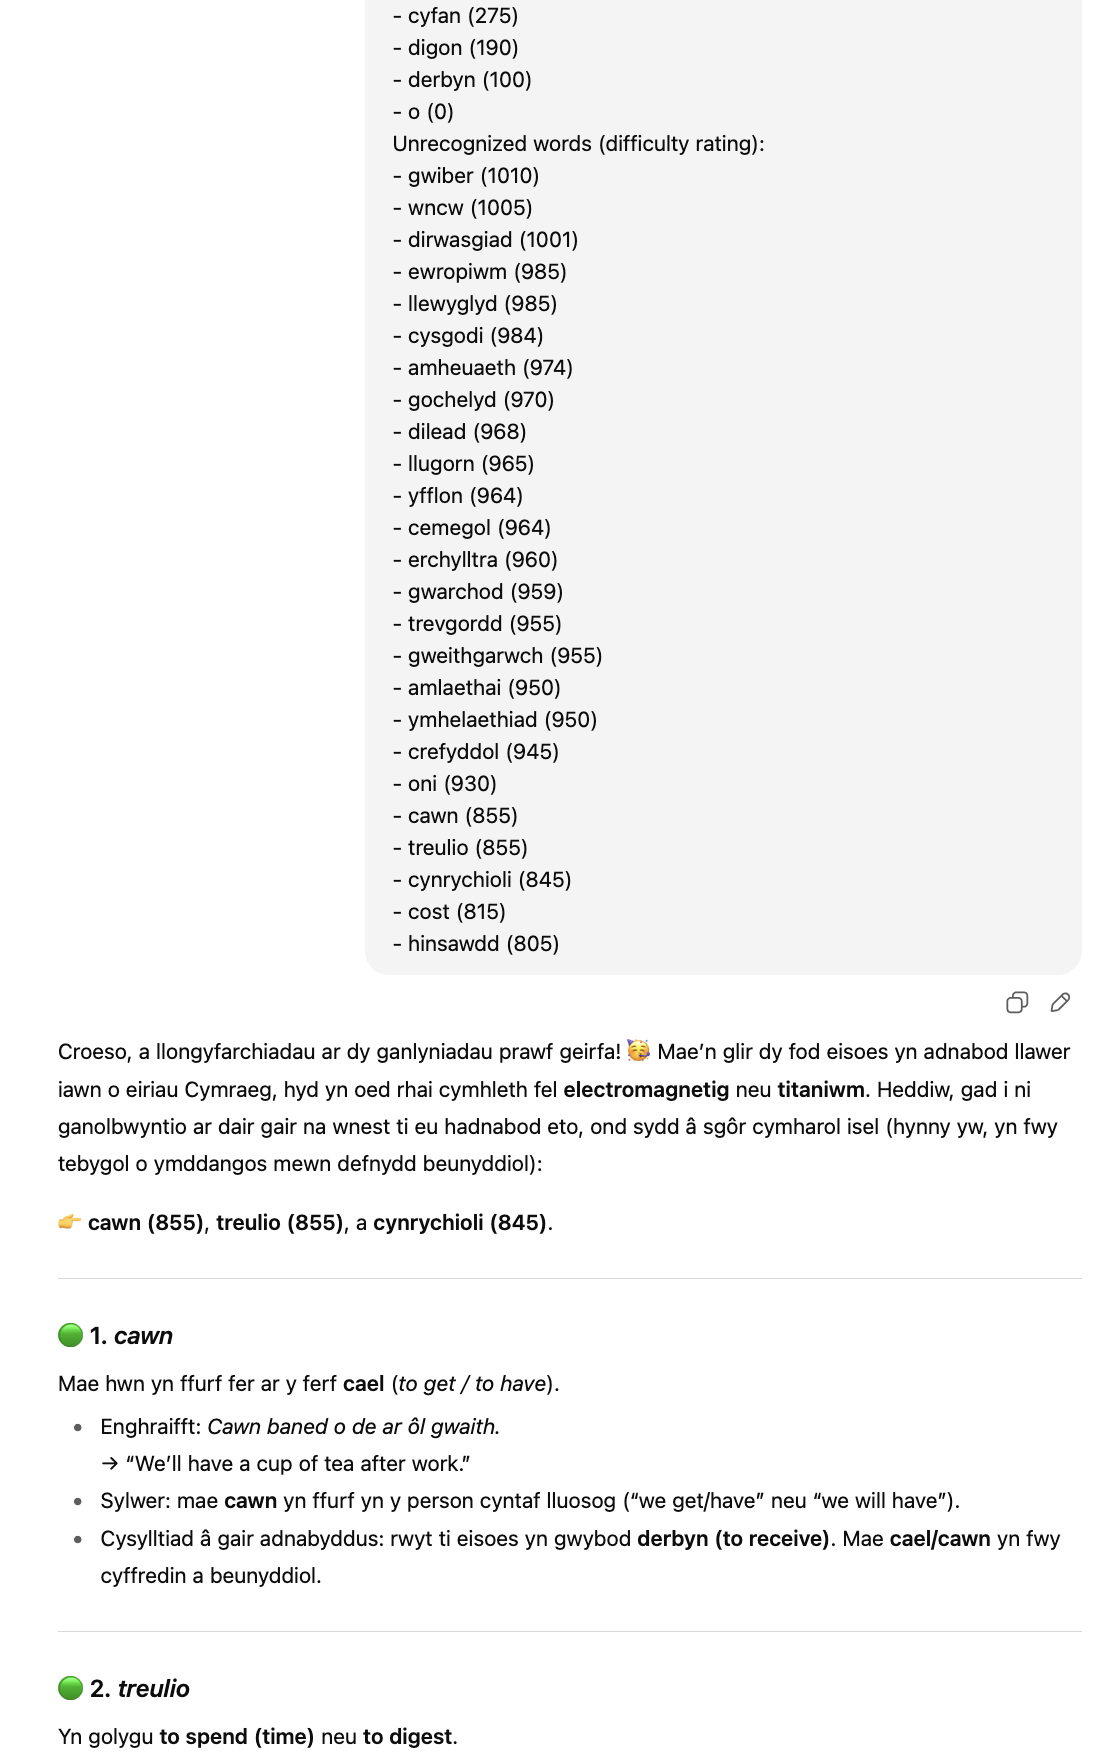
\includegraphics[width=0.8\textwidth]{figures/lesson-1.png}
    \caption{Beginning of a personalized lesson 1/2}
    \label{fig:lesson1}
\end{figure}
\begin{figure}[h]
    \centering
    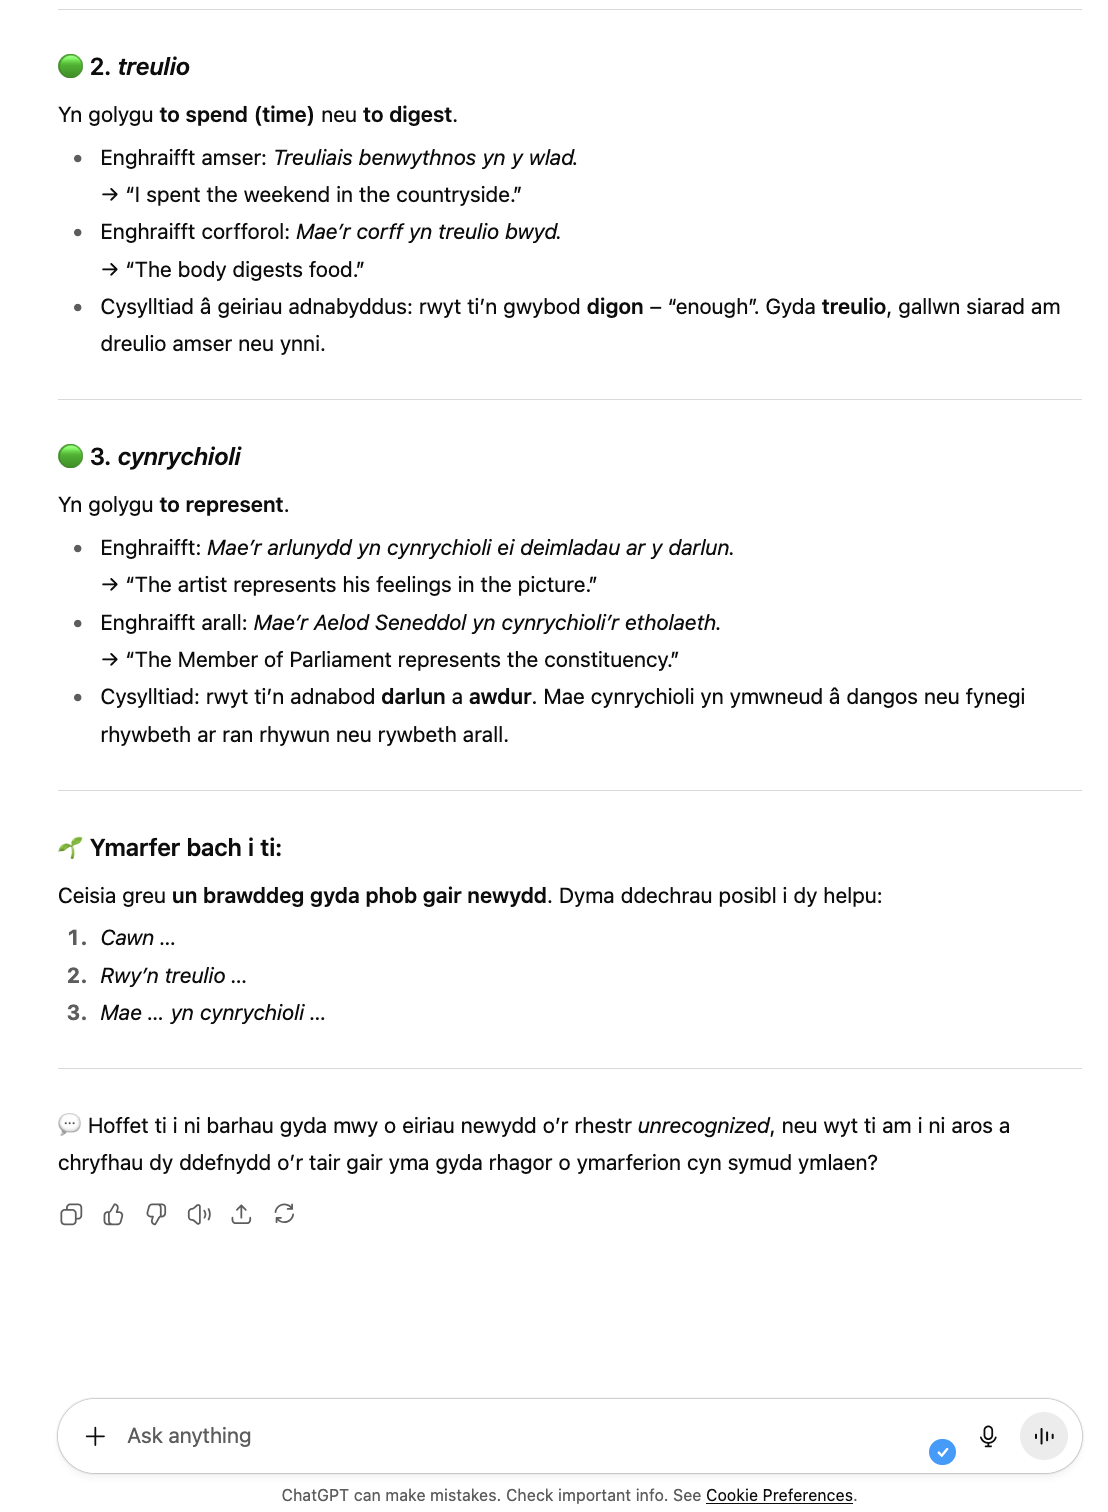
\includegraphics[width=0.8\textwidth]{figures/lesson-2.png}
    \caption{Beginning of a personalized lesson 2/2}
    \label{fig:lesson2}
    \medskip
    \small
    Indeed, ChatGPT can make mistakes, the word \textit{digon} is not mentioned anywhere, yet the second section implies it is present somewhere or that it is related in some way to the word \textit{treulio}. And \textit{gair} is masculine, so it should say \textit{tri gair} and not \textit{tair gair}. Interestingly however, the LLM seems to work out that the the lowest rated words proper, within the 800-850 rating range, may have been missed by mistake and start its lesson by the fourth to the sixth lowest rated unrecognised words.
\end{figure}

    \end{appendices}

    \printbibliography
\end{document}
